\documentclass[12pt,a4paper]{article}
\usepackage[margin=2.5cm,headheight=15pt]{geometry}
\usepackage{newtxtext,newtxmath}
\usepackage{graphicx,booktabs,amsmath,float,caption,xcolor,listings,enumitem,array}
\usepackage{tikz}
\usetikzlibrary{arrows.meta,positioning,shapes.geometric}
\usepackage{setspace,titlesec,fancyhdr,tocloft}
\usepackage[hidelinks]{hyperref}
\graphicspath{{figs/}}
\captionsetup{font={small,it},labelfont={bf,it},labelsep=period}
\captionsetup[table]{position=top}
\setlength{\parskip}{0.6em}
\setlength{\parindent}{0pt}
\onehalfspacing
\emergencystretch=3em

% ---- format: "Section N - Title" headings, running title, centred page number
\newcommand{\shorttitle}{Image Preprocessing Pipeline for Plant Pest Detection}
\newcommand{\secword}{Section}
\titleformat{\section}{\Large\bfseries}{\secword\ \thesection\ -}{0.35em}{}
\titleformat{\subsection}{\large\bfseries}{\thesubsection}{0.5em}{}
\let\oldsection\section
\renewcommand{\section}{\clearpage\oldsection}
\pagestyle{fancy}
\fancyhf{}
\fancyhead[R]{\small\itshape\shorttitle}
\fancyfoot[C]{\thepage}
\renewcommand{\headrulewidth}{0.4pt}
\renewcommand{\cfttoctitlefont}{\Large\bfseries}
\renewcommand{\cftloftitlefont}{\Large\bfseries}
\renewcommand{\cftlottitlefont}{\Large\bfseries}
\renewcommand{\cftsecpresnum}{Section }
\renewcommand{\cftsecaftersnum}{ -}
\setlength{\cftsecnumwidth}{5.6em}
\setlength{\cftsubsecindent}{1.5em}
\renewcommand{\cftfigpresnum}{Figure }
\renewcommand{\cftfigaftersnum}{.}
\setlength{\cftfignumwidth}{5em}
\setlength{\cftfigindent}{0pt}
\renewcommand{\cfttabpresnum}{Table }
\renewcommand{\cfttabaftersnum}{.}
\setlength{\cfttabnumwidth}{5em}
\setlength{\cfttabindent}{0pt}
\newcommand{\frontsection}[1]{\clearpage\oldsection*{#1}\addcontentsline{toc}{subsection}{#1}}

\lstset{
  language=Python, basicstyle=\ttfamily\scriptsize, breaklines=true, columns=fullflexible,
  keywordstyle=\color{blue!60!black}, commentstyle=\color{green!40!black}, stringstyle=\color{red!55!black},
  numbers=left, numberstyle=\tiny\color{gray}, numbersep=6pt, frame=single, rulecolor=\color{black!20},
  showstringspaces=false, tabsize=4
}

\newcommand{\reporttitle}{Optimized Image Preprocessing and Feature Enhancement Pipeline for Plant Pest Detection}
\newcommand{\repourl}{https://github.com/shrayash25/dip-pest-preprocessing}

\begin{document}

\begin{titlepage}
\centering
\vspace*{0.3cm}
{\large A REPORT\par}
\vspace{0.5cm}
{\large ON\par}
\vspace{1.0cm}
{\LARGE\bfseries \reporttitle\par}
\vspace{1.0cm}
{\large BY\par}
\vspace{0.5cm}
{\large\bfseries Shrayash Barnwal\par 2023A3PS0361P\par}
\vspace{0.5cm}
{\large\bfseries Akshal Gondalia\par 2023B1A80856P\par}
\vspace{0.9cm}
{\normalsize Prepared for the course\par}
{\large\bfseries EEE F435 Digital Image Processing\par}
\vspace{1.0cm}

\includegraphics[width=3.0cm]{bits_logo}\par
\vspace{0.7cm}
{\large BIRLA INSTITUTE OF TECHNOLOGY AND SCIENCE, PILANI\par}
{\normalsize Semester I, Academic Year 2026-2027\par}
{\normalsize November 2026\par}
\end{titlepage}
\setcounter{page}{2}

\frontsection{Declaration}
We hereby declare that the work presented in this report entitled ``\reporttitle'' is an original piece of academic work carried out by us as the project of the course EEE F435 Digital Image Processing at the Birla Institute of Technology and Science, Pilani. The report has been prepared in fulfilment of the requirements of the course project for the academic year 2026-2027. All sources of information and references have been duly acknowledged.

We further declare that this report, in whole or in part, has not been submitted to any other institution or university for the award of any degree or diploma.

\vspace{1.5cm}
\begin{minipage}[t]{0.48\textwidth}
Shrayash Barnwal\\
2023A3PS0361P\\
BITS Pilani
\end{minipage}\hfill
\begin{minipage}[t]{0.48\textwidth}
Akshal Gondalia\\
2023B1A80856P\\
BITS Pilani
\end{minipage}

\vspace{0.8cm}
Date: 22nd November 2026

\frontsection{Acknowledgements}
We would like to express our sincere gratitude to the instructor and the teaching team of the course EEE F435 Digital Image Processing, BITS Pilani, for the project brief and for their guidance during the course. We thank S. Jia, M. Horri Rezaei and B. Honarvar Shakibaei Asli, whose paper is the reference for this project. We also thank the photographers who share their observations on iNaturalist under Creative Commons licences; their images are the dataset of this work, and each one is credited in the attribution file of the repository. Finally, we acknowledge the developers of the open-source libraries OpenCV, NumPy, scikit-image, scikit-learn and Matplotlib.

\frontsection{Abstract}
Raw field images of plant pests are large, differ in quality, and contain leaf background that is not useful to a classifier. This report describes a reproducible batch pipeline in Python and OpenCV for six pest classes: green aphid, yellow aphid, black aphid, whitefly, red mite and mealybug. The pipeline follows the central idea of the reference paper: measure image quality first, then select the restoration from the measurement. Each image is scored with the BRISQUE no-reference metric. A low-quality image is processed by six candidate filters (median, Gaussian, Wiener, Richardson--Lucy, total variation, unsharp masking) and the best result is kept; the paper made this selection by hand, and here it is automatic. The pipeline then masks the green leaf background (HSV range and Otsu threshold on the LAB chroma distance), applies CLAHE and sharpening, resizes with aspect-ratio padding to $512\times512$ and compresses to JPEG. On 590 images the dataset size fell from 566.2~MB to 30.7~MB (94.6\%) at a mean of 121~ms for each image. For the 128 low-quality images the mean BRISQUE score fell from 39.1 to 15.9, close to the 40.75 to 16.17 that the paper reports. A controlled test with known clean images showed that the BRISQUE-selected filter raised PSNR by 0.5~dB for blur, 5.1~dB for Gaussian noise and 15.9~dB for salt-and-pepper noise. An SVM classifier gained 1.4 percentage points (45.0\% to 46.4\%), which is a small effect. The main limitations are that almost all the storage gain comes from resizing and compression, and that a colour mask cannot separate a green pest from a green leaf.

\vspace{0.6em}
\textbf{Keywords:} image preprocessing, plant pest detection, BRISQUE, image restoration, background masking, Otsu threshold, CLAHE, image compression

\clearpage
\begin{singlespace}
\tableofcontents
\clearpage
\listoffigures
\vspace{1cm}
\listoftables
\end{singlespace}

% ==============================================================================
\section{Introduction}

\subsection{Problem statement}
Automatic pest identification depends on images that are taken in the field with phones and handheld cameras. Three properties of these images cause problems for a machine-learning model.
\begin{itemize}[nosep]
\item \textbf{Size.} A raw photo has several megapixels, while a classifier uses an input of a few hundred pixels on each side. Storing and loading the raw files wastes space and time.
\item \textbf{Variable quality.} Blur, sensor noise and uneven light hide the small textures (body segments, wax, hairs) that separate one pest from another.
\item \textbf{Irrelevant background.} Most pixels are healthy leaf. A model can learn the host plant in place of the pest.
\end{itemize}

\subsection{Motivation}
Jia et al.\ \cite{jia2025} argue that image quality management is a prerequisite for a detector and not an optional step. They score each image with no-reference quality metrics, restore the low-quality images with a filter chosen for each image, and then train a YOLOv5 detector. They state two limitations of their own work: the filter and its parameters were selected by hand, which does not scale, and the cost of trying many filters is high. This project implements their quality-first idea as an automatic batch process and adds the stages that a dataset needs before training: background masking, contrast enhancement, size normalisation and compression.

\subsection{Objectives}
\begin{enumerate}[nosep]
\item Build a batch script that runs from start to end with one command and writes size-reduced images into one folder for each of the six classes.
\item Implement the quality assessment and restoration stage of the reference paper, with automatic filter selection.
\item Segment out the healthy leaf background without losing pale or small pests.
\item Apply local contrast and edge enhancement.
\item Measure the storage reduction, the time for each image, and the quality before and after, and compare with baseline methods.
\item Test whether the processing helps a classifier.
\end{enumerate}

% ==============================================================================
\section{Theory}
\label{sec:theory}

\subsection{Image degradation model}
The reference paper \cite{jia2025} models an acquired image $g$ as an ideal image $f$ blurred by a point spread function (PSF) $h$ with additive noise $n$:
\begin{equation}
g(x,y) = f(x,y) * h(x,y) + n(x,y)
\quad\Longleftrightarrow\quad
G(u,v) = F(u,v)\,H(u,v) + N(u,v),
\label{eq:degradation}
\end{equation}
where $*$ is 2-D convolution and capital letters are Fourier transforms. Restoration estimates $f$ from $g$. Which filter is correct depends on which term dominates: a smoothing filter removes $n$, and a deconvolution filter inverts $h$. A wrong choice makes the image worse, which is why a quality measurement comes first.

\subsection{No-reference quality assessment: BRISQUE}
Field images have no clean reference, so full-reference metrics such as PSNR cannot be used on them. BRISQUE \cite{mittal2012} needs only the image. It calculates the mean-subtracted contrast-normalised (MSCN) coefficients
\begin{equation}
\hat{I}(i,j) = \frac{I(i,j) - \mu(i,j)}{\sigma(i,j) + C},
\end{equation}
where $\mu$ and $\sigma$ are the local mean and standard deviation in a Gaussian window and $C$ is a small constant. For a natural, undistorted image the histogram of $\hat{I}$ is close to a Gaussian. Blur makes it more peaked and noise makes it flatter. BRISQUE fits a generalised Gaussian distribution to $\hat{I}$ and asymmetric generalised Gaussians to the products of neighbouring coefficients in four directions, at two scales. This gives 36 features, and a support vector regressor trained on human opinion scores maps them to one score. A lower score means better quality; the reference paper treats images below 30 as good.

\subsection{Restoration filters}
\label{sec:filters}
\paragraph{Median filter.} Each pixel is replaced by the median of its $k\times k$ neighbourhood. An impulse (salt-and-pepper) pixel is an outlier in the sorted window and is never selected, so the filter removes impulse noise and keeps edges better than a linear filter.

\paragraph{Gaussian filter.} The image is convolved with $G_\sigma(x,y)=\frac{1}{2\pi\sigma^2}\exp\!\left(-\frac{x^2+y^2}{2\sigma^2}\right)$. It is a low-pass filter that reduces zero-mean sensor noise, at the cost of some blur.

\paragraph{Wiener filter.} The Wiener filter minimises the mean square error between the estimate and the ideal image. With a constant noise-to-signal power ratio $K = S_n/S_f$ it is
\begin{equation}
\hat{F}(u,v) = \frac{H^{*}(u,v)}{|H(u,v)|^{2} + K}\; G(u,v).
\label{eq:wiener}
\end{equation}
Where $|H|^2 \gg K$ it acts as an inverse filter and restores detail; where $|H|^2 \ll K$ it attenuates, so noise is not amplified.

\paragraph{Richardson--Lucy deconvolution.} This is an iterative maximum-likelihood estimate for Poisson noise \cite{richardson1972,lucy1974}:
\begin{equation}
\hat{f}_{k+1} = \hat{f}_k \cdot \left[\, h^{\star} * \frac{g}{h * \hat{f}_k} \,\right],
\end{equation}
where $h^{\star}$ is the flipped PSF. The estimate stays non-negative, and the number of iterations controls the trade-off between sharpness and noise amplification.

\paragraph{Total variation denoising.} The Rudin--Osher--Fatemi model \cite{rudin1992,chambolle2004} finds
\begin{equation}
\hat{f} = \arg\min_{f}\; \tfrac{1}{2}\,\lVert f - g\rVert_2^2 + \lambda \int \lvert\nabla f\rvert \, dx\,dy .
\end{equation}
The penalty is on the total gradient magnitude and not on its square, so flat regions are smoothed while step edges stay sharp.

\paragraph{Unsharp masking.} $f_s = f + a\,(f - G_\sigma * f)$ adds back the high-frequency part of the image with gain $a$. It increases edge contrast but also amplifies noise.

\subsection{Colour spaces}
RGB mixes brightness and colour in all three channels, which makes colour thresholds sensitive to lighting. Two other spaces are used.
\begin{itemize}[nosep]
\item \textbf{HSV} separates hue $H$ (the colour angle), saturation $S$ and value $V$. A leaf is selected with a range of $H$, almost independent of how bright it is.
\item \textbf{CIELAB} separates lightness $L^*$ from two colour-opponent axes: $a^*$ (green to red) and $b^*$ (blue to yellow). Euclidean distance in the $(a^*,b^*)$ plane is close to the perceived colour difference. Enhancement on $L^*$ alone changes contrast and does not shift colours.
\end{itemize}

\subsection{Otsu's threshold}
Otsu's method \cite{otsu1979} selects the threshold $t$ that maximises the between-class variance of a histogram with class probabilities $\omega_0(t),\omega_1(t)$ and class means $\mu_0(t),\mu_1(t)$:
\begin{equation}
\sigma_B^2(t) = \omega_0(t)\,\omega_1(t)\,\bigl[\mu_0(t) - \mu_1(t)\bigr]^2,
\qquad t^{*} = \arg\max_t\, \sigma_B^2(t).
\end{equation}
It needs no manual parameter. It always returns a threshold, even for a histogram with one mode, so the result must be bounded when one class may be absent.

\subsection{Morphological operations}
For a binary mask $A$ and a structuring element $B$, erosion $A\ominus B$ shrinks regions and dilation $A\oplus B$ grows them. Opening $(A\ominus B)\oplus B$ removes regions smaller than $B$, and closing $(A\oplus B)\ominus B$ fills holes smaller than $B$. Connected-component labelling gives the area of each region, so regions below an area limit can be removed.

\subsection{Contrast limited adaptive histogram equalisation}
Global histogram equalisation maps grey level $r$ through the cumulative distribution, $s = (L-1)\sum_{j\le r} p(j)$. One mapping for the full image over-amplifies large uniform areas. CLAHE \cite{zuiderveld1994} divides the image into tiles and equalises each tile, with two changes: the tile histogram is clipped at a limit and the excess is redistributed, which bounds the slope of the mapping and therefore the noise amplification; and the mappings of adjacent tiles are bilinearly interpolated, which removes tile borders.

\subsection{Resizing, bit depth and compression}
An $H\times W$ image is scaled by $s = T/\max(H,W)$ and centred on a $T\times T$ canvas with zero padding. The aspect ratio is kept, so the shape of the pest is not distorted. Area interpolation is used for reduction because it averages the source pixels and so prevents aliasing. A 16-bit image is scaled to 8 bits by $I_8 = \mathrm{round}(I_{16}/257)$, which maps $65535$ to $255$ exactly.

JPEG converts to YCbCr, subsamples the chroma channels, applies the discrete cosine transform to $8\times8$ blocks, quantises the coefficients and entropy-codes them. Quantisation removes high-frequency coefficients, so a smooth image compresses more. A masked background is constant, so it costs almost no bits.

\subsection{Evaluation metrics}
With grey image $I$, mean $\bar{I}$ and histogram $p$:
\begin{align}
\text{RMS contrast} &= \sqrt{\tfrac{1}{N}\textstyle\sum (I - \bar{I})^2}, &
\text{Entropy} &= -\textstyle\sum_{k} p(k)\log_2 p(k), \\
\text{Sharpness} &= \mathrm{Var}\bigl(\nabla^2 I\bigr), &
\text{PSNR} &= 10\log_{10}\frac{255^2}{\mathrm{MSE}(f,\hat{f})}.
\end{align}
SSIM \cite{wang2004} compares local luminance, contrast and structure between a reference and a test image and is 1 for identical images. PSNR and SSIM need a reference image; the other metrics and BRISQUE do not.

\section{Methodology}
\label{sec:method}

\subsection{Dataset}
The course dataset was not available when this work was done, so a public stand-in dataset with the same six classes was assembled. No single public dataset contains all six classes. The images are research-grade observations from iNaturalist \cite{inaturalist} with Creative Commons licences; ``research-grade'' means that the species identification was confirmed by more than one person. One photo was taken from each observation to avoid near-duplicate frames, and photos with a short side below 800 pixels were skipped. Table~\ref{tab:dataset} lists the classes. The download script writes a manifest with the photographer, licence and source page of each image, and later runs read that manifest, so the dataset is reproducible.

\begin{table}[H]
\centering
\caption{Stand-in dataset. All images are field photographs with uncontrolled lighting and background.}
\label{tab:dataset}
\begin{tabular}{llr}
\toprule
Class & Taxon used & Images \\
\midrule
Green aphid  & \textit{Myzus persicae}, \textit{Acyrthosiphon pisum} & 90 \\
Yellow aphid & \textit{Aphis nerii} & 100 \\
Black aphid  & \textit{Aphis fabae} complex & 100 \\
Whitefly     & family Aleyrodidae & 100 \\
Red mite     & genus \textit{Tetranychus} & 100 \\
Mealybug     & family Pseudococcidae & 100 \\
\midrule
Total & & 590 \\
\bottomrule
\end{tabular}
\end{table}

\subsection{Pipeline}
Figure~\ref{fig:flowchart} shows the pipeline. Each image goes through seven stages.

\begin{figure}[H]
\centering
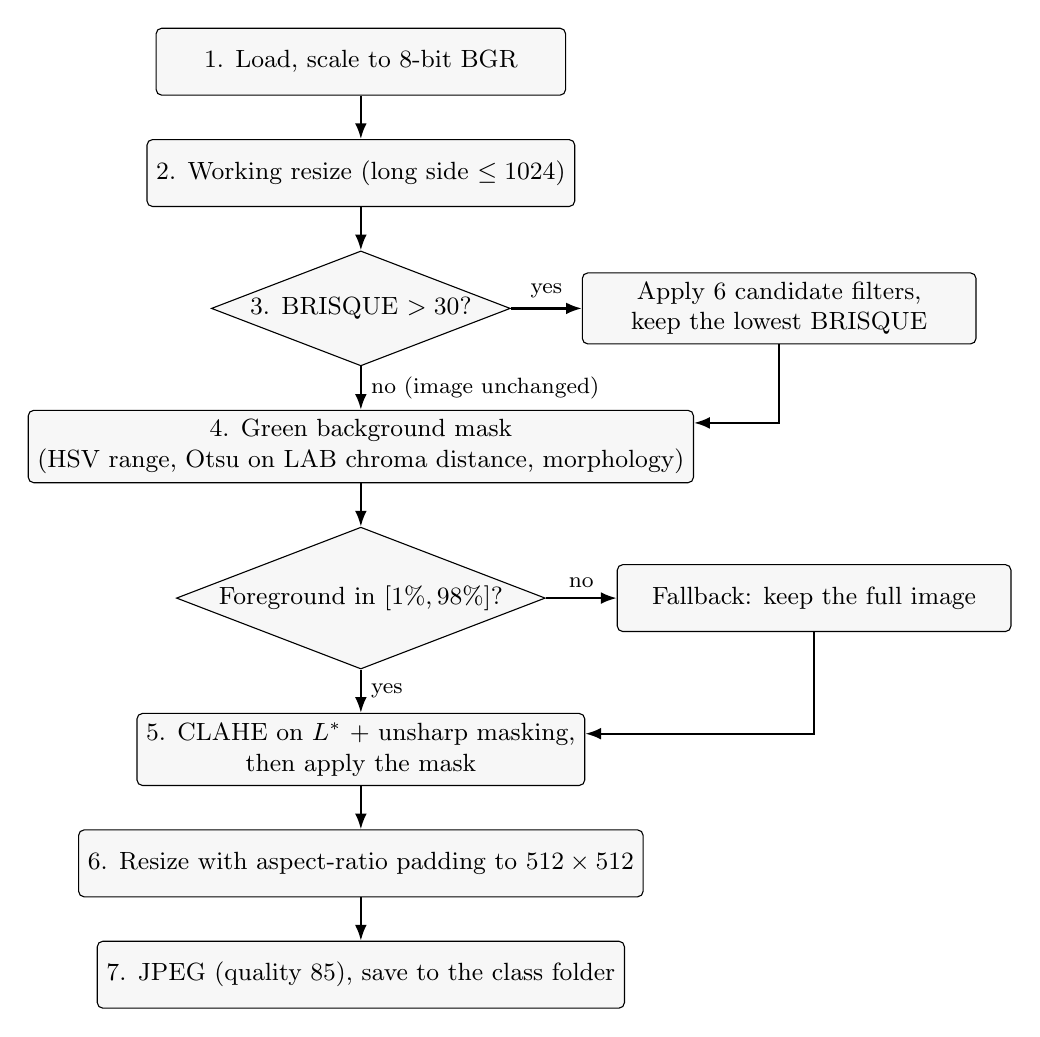
\begin{tikzpicture}[
  node distance=5.5mm and 9mm,
  box/.style={draw, rounded corners=2pt, align=center, minimum width=52mm, minimum height=8.5mm, font=\small, fill=black!3},
  dec/.style={draw, diamond, aspect=2.6, align=center, inner sep=1pt, font=\small, fill=black!3},
  side/.style={draw, rounded corners=2pt, align=center, minimum width=50mm, minimum height=8.5mm, font=\small, fill=black!3},
  arr/.style={-{Latex[length=2mm]}, thick},
  lab/.style={font=\footnotesize}
]
\node[box] (load) {1. Load, scale to 8-bit BGR};
\node[box, below=of load] (work) {2. Working resize (long side $\le 1024$)};
\node[dec, below=of work] (iqa) {3. BRISQUE $> 30$?};
\node[side, right=of iqa] (restore) {Apply 6 candidate filters,\\keep the lowest BRISQUE};
\node[box, below=of iqa] (mask) {4. Green background mask\\(HSV range, Otsu on LAB chroma distance, morphology)};
\node[dec, below=of mask] (fb) {Foreground in $[1\%, 98\%]$?};
\node[side, right=of fb] (keep) {Fallback: keep the full image};
\node[box, below=of fb] (clahe) {5. CLAHE on $L^*$ + unsharp masking,\\then apply the mask};
\node[box, below=of clahe] (resize) {6. Resize with aspect-ratio padding to $512\times512$};
\node[box, below=of resize] (save) {7. JPEG (quality 85), save to the class folder};
\draw[arr] (load) -- (work);
\draw[arr] (work) -- (iqa);
\draw[arr] (iqa) -- node[lab, above] {yes} (restore);
\draw[arr] (iqa) -- node[lab, right] {no (image unchanged)} (mask);
\draw[arr] (restore.south) |- ([yshift=3mm]mask.east);
\draw[arr] (mask) -- (fb);
\draw[arr] (fb) -- node[lab, above] {no} (keep);
\draw[arr] (fb) -- node[lab, right] {yes} (clahe);
\draw[arr] (keep.south) |- ([yshift=2mm]clahe.east);
\draw[arr] (clahe) -- (resize);
\draw[arr] (resize) -- (save);
\end{tikzpicture}
\caption{Algorithm flowchart of the preprocessing pipeline.}
\label{fig:flowchart}
\end{figure}

\paragraph{Stages 1--2: load and normalise.} The image is read with its original bit depth, scaled to 8 bits and converted to three channels. It is then reduced so that its long side is at most 1024 pixels. Masking and enhancement run at this working resolution, which keeps small pests visible and makes the time per image predictable.

\paragraph{Stage 3: quality check and restoration.} This stage follows the reference paper. The BRISQUE score of the image is calculated. If it is at most 30, the image is not changed. If it is above 30, six candidate filters are applied (median, Gaussian, Wiener, Richardson--Lucy, total variation, unsharp masking), BRISQUE is calculated for each result, and the result with the lowest score is kept. The unchanged image is also a candidate, so this stage cannot make the score worse. In the paper the filter and its parameters were selected by hand for each image; here the selection is automatic, which is the first future-work item that the authors list. The smoothing filters use the colour image because noise is in all channels. The deblurring filters use only $L^*$ so that they do not make colour fringes. The PSF is not known for a field photo, so a Gaussian PSF is assumed.

\paragraph{Stage 4: green background mask.} A plain HSV green range removes every green pixel, which also removes pests that are pale, translucent or green and pick up the colour of the leaf. The mask therefore has three steps.
\begin{enumerate}[nosep]
\item \textbf{HSV range.} After a Gaussian pre-smoothing, pixels with a green hue are the candidate leaf pixels. If fewer than 2\% of pixels are candidates, there is no leaf background and the image is kept as it is.
\item \textbf{Dominant leaf colour.} The median $(a^*, b^*)$ of the candidates is the dominant leaf colour. The chroma distance $d = \sqrt{(a^*-a^*_{m})^2 + (b^*-b^*_{m})^2}$ of each pixel from it is calculated.
\item \textbf{Otsu threshold.} Otsu's method on $d$, over the candidates only, separates ``leaf'' (near the dominant colour) from ``other'' (a pest with a green tint, a vein, a highlight). The threshold is limited to $[8, 25]$: below 8 a leaf with one colour mode would be split in two, and above 25 a clearly different colour would be removed.
\end{enumerate}
The background is the candidates with $d$ below the threshold. Opening and closing clean it, regions and holes smaller than 0.03\% of the image are removed, and the foreground is dilated to keep a margin around the pest. If the foreground is less than 1\% or more than 98\% of the image, the mask is not applied.

\paragraph{Stage 5: enhancement.} CLAHE is applied to $L^*$, followed by unsharp masking on $L^*$. The mask is then applied and the background becomes black.

\paragraph{Stages 6--7: resize and compress.} The result is resized with aspect-ratio padding to $512\times512$ and saved as an 8-bit JPEG in the folder of its class.

\subsection{Parameter settings}
Table~\ref{tab:params} gives all parameters. They are constants at the top of the script.

\begin{table}[H]
\centering
\caption{Parameter settings.}
\label{tab:params}
\small
\begin{tabular}{lll}
\toprule
Stage & Parameter & Value \\
\midrule
Resize & Working long side; output size & 1024 px; $512\times512$ \\
Quality check & BRISQUE threshold & 30 (from \cite{jia2025}) \\
Median filter & Window & $3\times3$ \\
Gaussian filter & $\sigma$ & 1.0 \\
Wiener filter & Gaussian PSF $\sigma$; $K$ & 1.2; 0.02 \\
Richardson--Lucy & Gaussian PSF $\sigma$; iterations & 1.2; 10 \\
Total variation & Weight $\lambda$ & 0.10 \\
Sharpening candidate & $\sigma$; gain $a$ & 1.0; 1.0 \\
Mask & Pre-smoothing $\sigma$ & 2.0 \\
Mask & HSV green range (OpenCV scale) & $H\in[35,90]$, $S\ge30$, $V\ge40$ \\
Mask & Chroma distance threshold & Otsu, limited to $[8,25]$ \\
Mask & Opening; closing; dilation (ellipse) & $5\times5$; $9\times9$; $7\times7$ \\
Mask & Minimum region area & 0.03\% of the image \\
Mask & Foreground limits for the fallback & 1\% and 98\% \\
CLAHE & Clip limit; tile grid & 2.0; $8\times8$ \\
Unsharp masking & $\sigma$; gain $a$ & 1.0; 0.6 \\
Compression & JPEG quality & 85 \\
\bottomrule
\end{tabular}
\end{table}

\subsection{Experiments}
\label{sec:experiments}
Four experiments measure the pipeline.
\begin{enumerate}[nosep]
\item \textbf{Storage and time.} Raw and processed size for each class, and the time of each stage for each image.
\item \textbf{Baseline comparison.} Five versions of each image at the same output size: (A) resize only, (B) global histogram equalisation, (C) CLAHE only, (D) restoration + CLAHE + sharpening without the mask, (E) the full pipeline. Contrast, entropy, sharpness, BRISQUE and compressed size are compared. For version E the metrics use only the foreground pixels, and BRISQUE is not reported because a black background is not a natural image.
\item \textbf{Controlled degradation.} BRISQUE selects the filter, so a BRISQUE improvement alone does not prove that the selected filter is correct. Sixty clean images (BRISQUE $\le 20$, ten for each class) are degraded with Gaussian blur ($\sigma = 1.5$), Gaussian noise ($\sigma = 15$ grey levels) and 4\% salt-and-pepper noise. Each filter is applied and PSNR and SSIM are measured against the clean image.
\item \textbf{Classifier.} An RBF support vector machine is trained on colour histograms (HSV) and texture histograms (local binary patterns) from versions A, C, D and E, with stratified 5-fold cross-validation repeated three times. All versions use the same folds.
\end{enumerate}


% ==============================================================================
\section{Implementation}

\subsection{Software}
The project is in Python 3.13 with OpenCV 5.1 (contrib build, for the BRISQUE module), NumPy 2.5, scikit-image 0.26, scikit-learn 1.9 and Matplotlib 3.11 \cite{opencv,scikit-image,scikit-learn}. Exact versions are pinned in \texttt{requirements.txt}. All measurements were made on a laptop with an Apple M4 processor and 16~GB of memory, on the CPU only. The code is available at \url{\repourl}.

\subsection{Program structure}
\begin{table}[H]
\centering
\caption{Scripts.}
\small
\begin{tabular}{ll}
\toprule
File & Purpose \\
\midrule
\texttt{run\_all.py} & Runs all the steps in order with one command \\
\texttt{download\_dataset.py} & Downloads the dataset and writes the attribution manifest \\
\texttt{pest\_pipeline.py} & Pipeline stages, batch run, metrics and summary tables \\
\texttt{figures.py} & Step plots and charts \\
\texttt{degradation\_experiment.py} & Controlled degradation test (PSNR, SSIM) \\
\texttt{classify\_eval.py} & SVM comparison of raw and processed images \\
\bottomrule
\end{tabular}
\end{table}

\subsection{Main functions}
Table~\ref{tab:functions} lists the functions that implement each stage in \texttt{pest\_pipeline.py}.

\begin{table}[H]
\centering
\caption{Functions for each processing stage.}
\label{tab:functions}
\small
\begin{tabular}{p{4.6cm}p{10.4cm}}
\toprule
Function & Processing step \\
\midrule
\texttt{load\_image} & Reads the file; scales 16-bit data to 8-bit; converts grey or BGRA to BGR \\
\texttt{limit\_long\_side} & Area-interpolation resize to the working resolution \\
\texttt{brisque\_score} & BRISQUE score with the OpenCV quality module \\
\texttt{wiener\_deconvolve} & Wiener filter, Eq.~\eqref{eq:wiener}, with the FFT; reflect padding reduces ringing at the borders \\
\texttt{richardson\_lucy} & Richardson--Lucy iterations with a Gaussian PSF \\
\texttt{total\_variation}, \texttt{sharpen\_filter} & Total variation denoising; unsharp masking \\
\texttt{iqa\_guided\_restore} & Scores the image, applies the candidates if needed, keeps the lowest score \\
\texttt{otsu\_threshold} & Otsu's method from the histogram, written in NumPy; also returns the separability $\sigma_B^2/\sigma_T^2$ \\
\texttt{green\_background\_mask} & HSV range, dominant leaf colour, Otsu on the chroma distance, morphology, region filter, fallback \\
\texttt{clahe\_on\_lightness} & CLAHE on $L^*$ and unsharp masking \\
\texttt{letterbox} & Resize with aspect-ratio padding \\
\texttt{encode\_jpeg} & JPEG compression at quality 85 \\
\texttt{quality\_metrics} & Brightness, RMS contrast, entropy and Laplacian variance inside a region \\
\bottomrule
\end{tabular}
\end{table}

Three implementation points matter for the results.
\begin{itemize}[nosep]
\item \textbf{Fair metrics.} Padding and masked background are black. If they were included, contrast and entropy would change for reasons that have nothing to do with enhancement. All quality metrics are therefore calculated only inside the image content, and for the masked output only inside the foreground.
\item \textbf{Fair timing.} One image is processed before timing starts, because the first OpenCV call includes start-up cost. Each stage is timed separately, and the baseline measurements are not included in the pipeline time.
\item \textbf{Reproducibility.} File lists are sorted, random seeds are fixed, and the dataset is defined by a manifest file. Running \texttt{python run\_all.py} recreates every table and figure in this report.
\end{itemize}

% ==============================================================================
\section{Results}

\subsection{Processing stages}
Figure~\ref{fig:steps} shows one image of each class at each stage. The mask keeps the pests and removes the leaf in the yellow aphid, black aphid, mealybug and whitefly examples. Where the image has no green background, or where the mask would keep less than 1\% or more than 98\% of the image, the mask is not applied and the full image is kept (a white mask).

\begin{figure}[H]
\centering
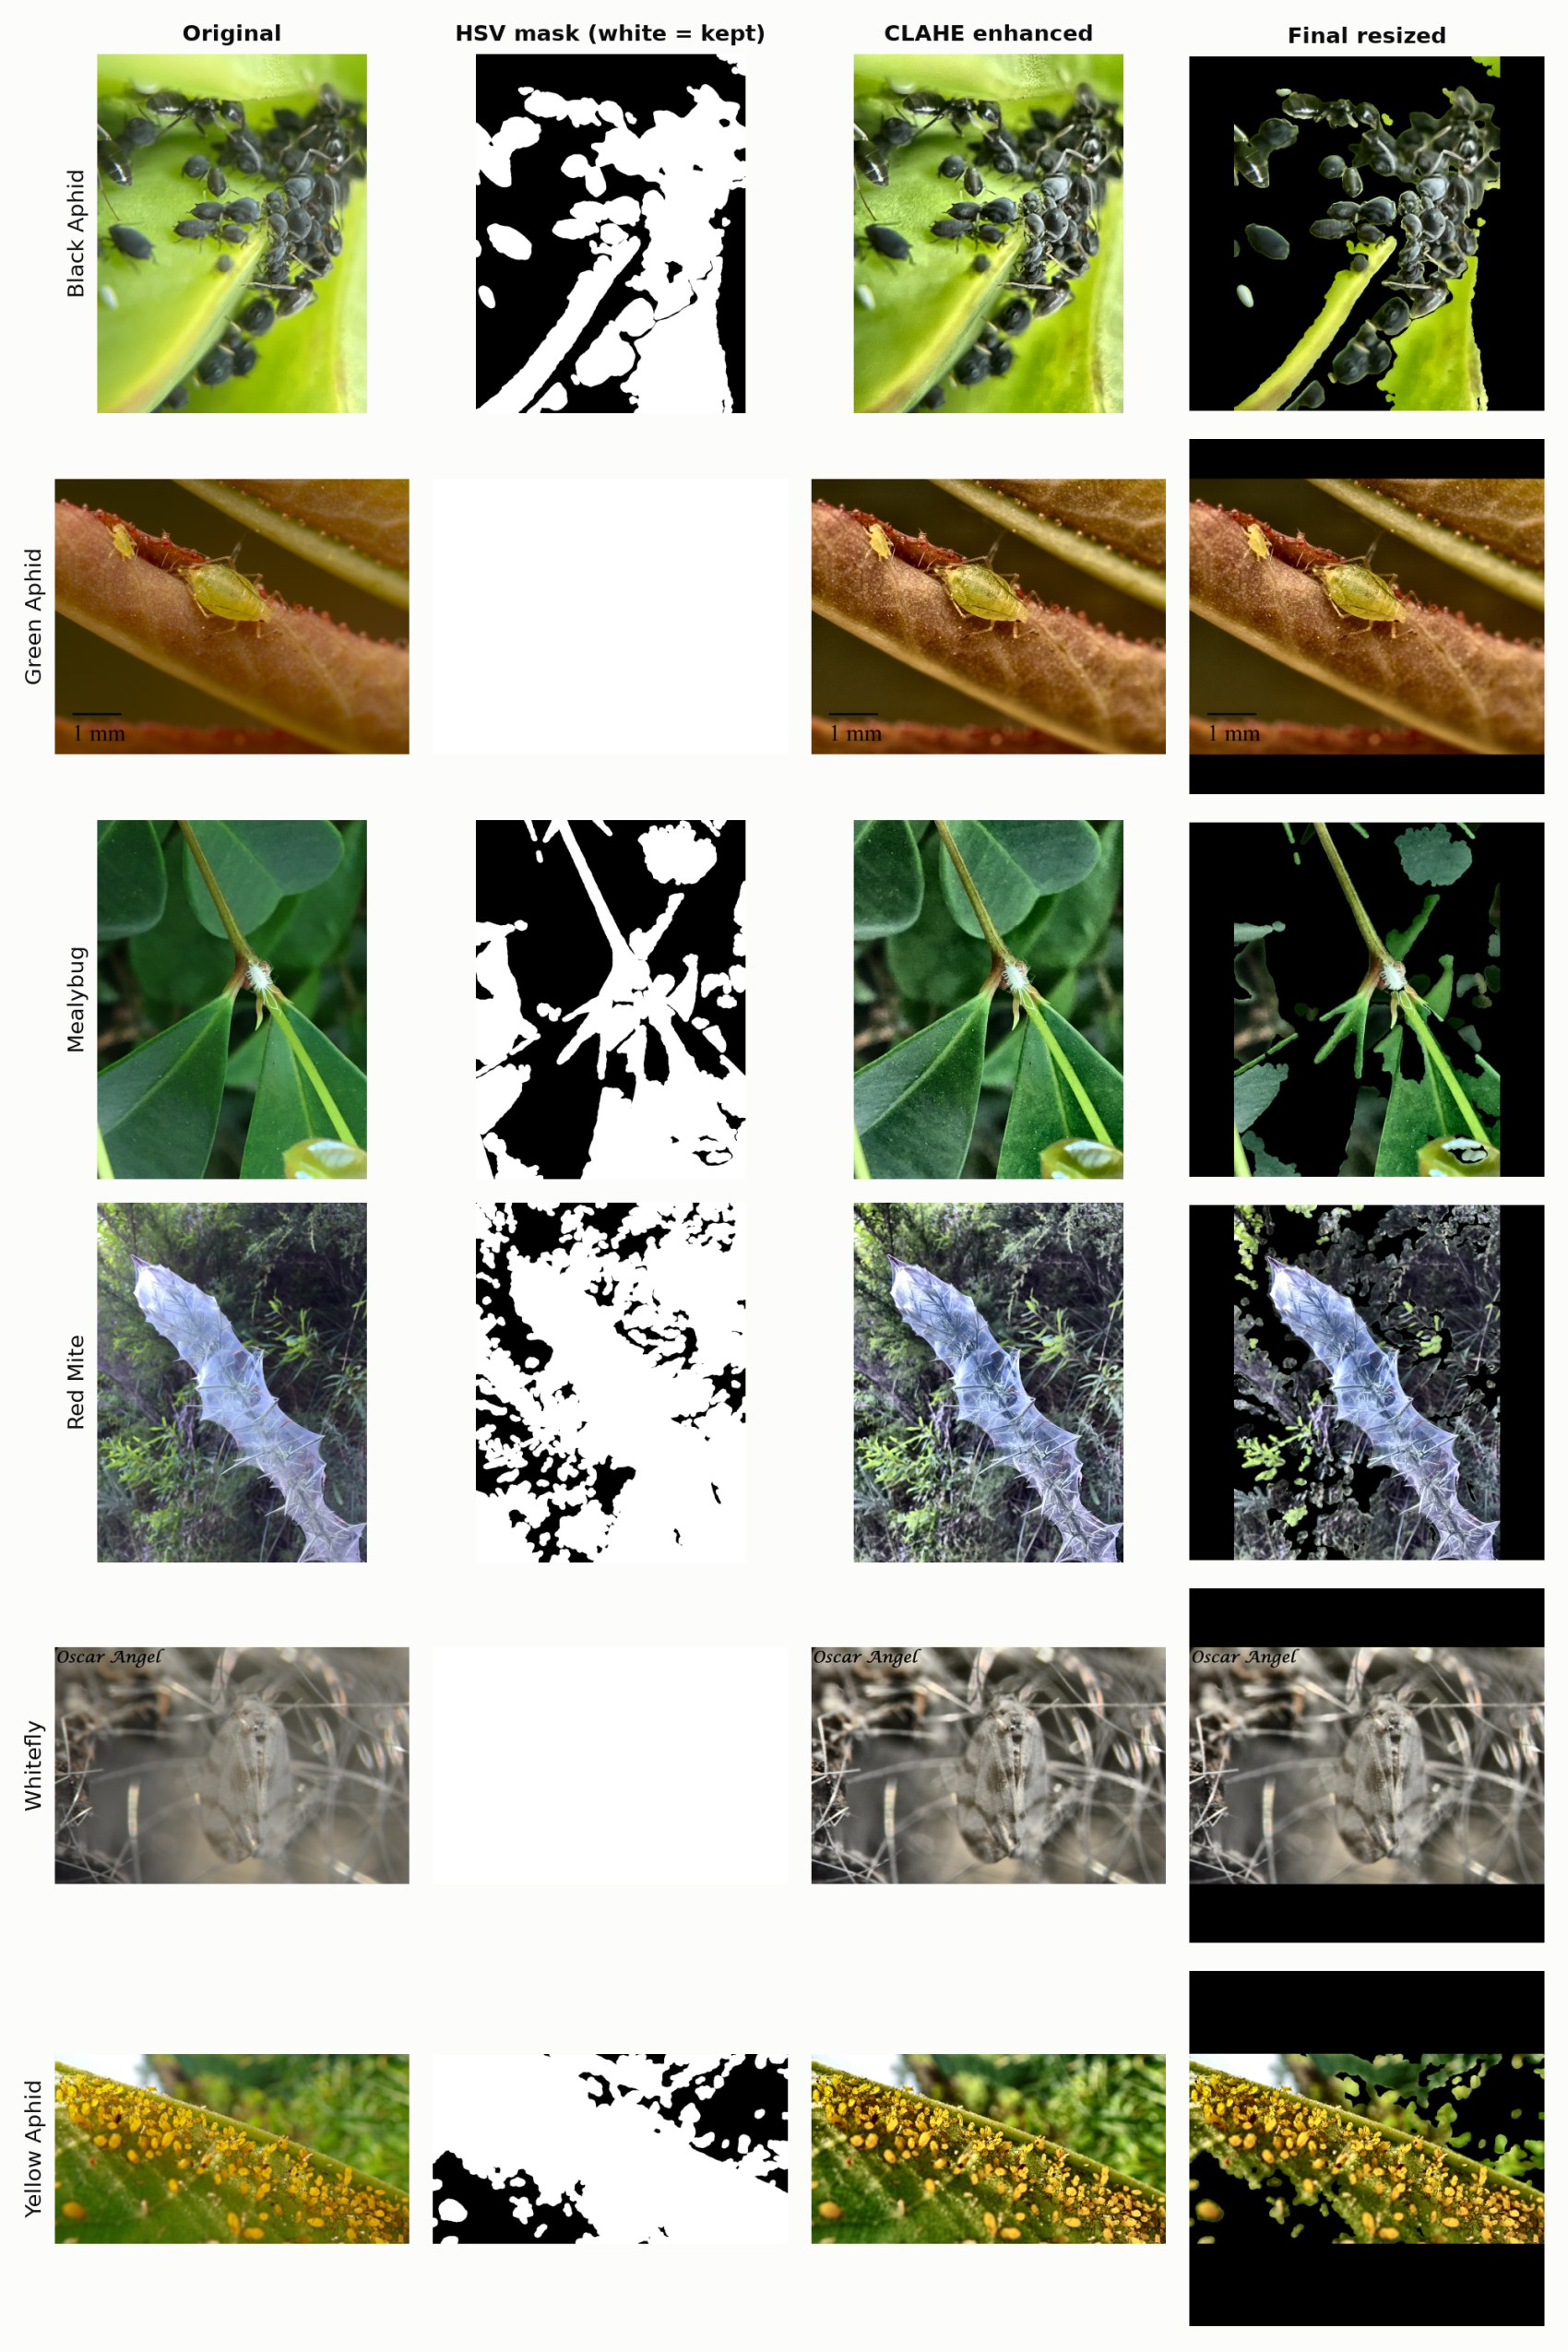
\includegraphics[width=0.74\textwidth]{steps_overview.jpg}
\caption{Processing steps for one image of each class: original, foreground mask, enhanced image, and final $512\times512$ output.}
\label{fig:steps}
\end{figure}

\subsection{Storage reduction}
Table~\ref{tab:storage} and Figure~\ref{fig:storage} give the storage result. The dataset fell from 566.2~MB to 30.7~MB, a reduction of 94.6\% (ratio 18.4). The mean file size fell from 983~kB to 53~kB.

\begin{table}[H]
\centering
\caption{Storage footprint and mean processing time for each class.}
\label{tab:storage}
\small
\begin{tabular}{lrrrrrr}
\toprule
Class & Images & Raw (MB) & Processed (MB) & Reduction (\%) & Ratio & Time (ms/image) \\
\midrule
Black aphid  & 100 &  84.64 & 4.95 & 94.15 & 17.1 & 146.6 \\
Green aphid  &  90 &  98.42 & 3.94 & 96.00 & 25.0 & 124.8 \\
Mealybug     & 100 &  82.18 & 4.98 & 93.94 & 16.5 & 107.8 \\
Red mite     & 100 & 113.40 & 6.67 & 94.11 & 17.0 &  97.6 \\
Whitefly     & 100 &  95.99 & 5.04 & 94.75 & 19.1 & 110.2 \\
Yellow aphid & 100 &  91.61 & 5.15 & 94.37 & 17.8 & 138.4 \\
\midrule
Total        & 590 & 566.23 & 30.73 & 94.57 & 18.4 & 120.8 \\
\bottomrule
\end{tabular}
\end{table}

\begin{figure}[H]
\centering
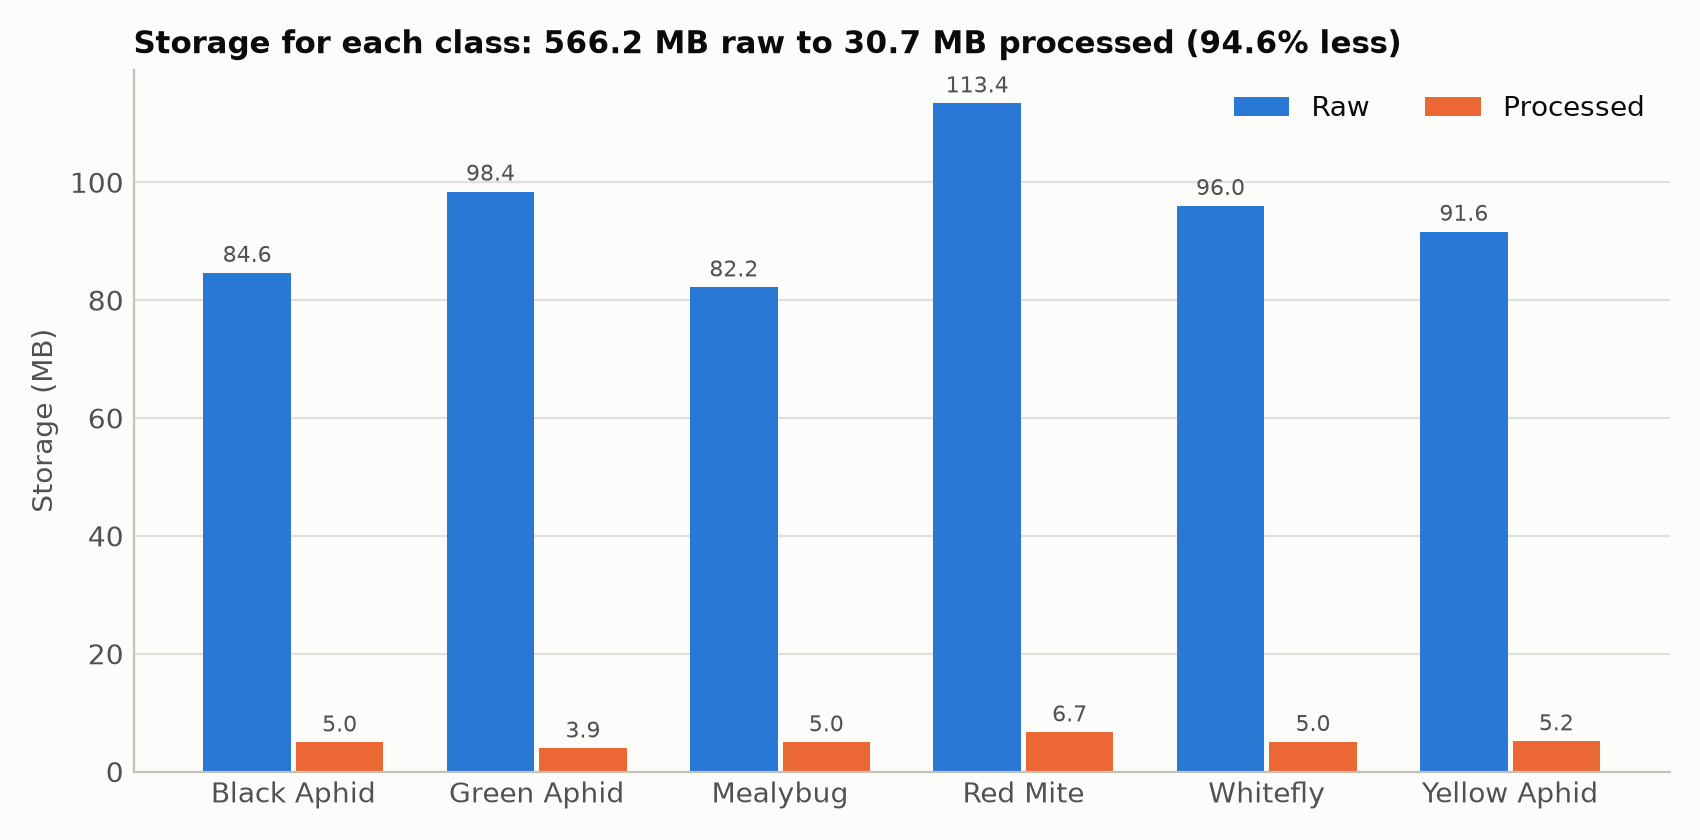
\includegraphics[width=0.72\textwidth]{storage_per_class.png}
\caption{Raw and processed storage for each class.}
\label{fig:storage}
\end{figure}

\subsection{Execution time}
The mean time is 120.8~ms for each image and the median is 46.0~ms (Table~\ref{tab:timing}, Figure~\ref{fig:timing}). The distribution has two groups. An image that passes the quality check takes 45~ms on average. An image that is flagged takes 395~ms, because six filters and six more BRISQUE scores are calculated. The 22\% of images that are flagged account for most of the total time.

\begin{table}[H]
\centering
\caption{Mean time for each stage (590 images).}
\label{tab:timing}
\small
\begin{tabular}{lrr}
\toprule
Stage & Mean (ms) & Std.\ dev.\ (ms) \\
\midrule
Load and decode & 9.15 & 4.31 \\
Working resize & 1.08 & 1.04 \\
Quality check and restoration & 97.81 & 154.53 \\
Green background mask & 9.40 & 3.68 \\
CLAHE and sharpening & 1.61 & 0.28 \\
Final resize and padding & 0.29 & 0.33 \\
JPEG encode and write & 1.46 & 0.29 \\
\midrule
Total & 120.81 & 153.43 \\
\bottomrule
\end{tabular}
\end{table}

\begin{figure}[H]
\centering
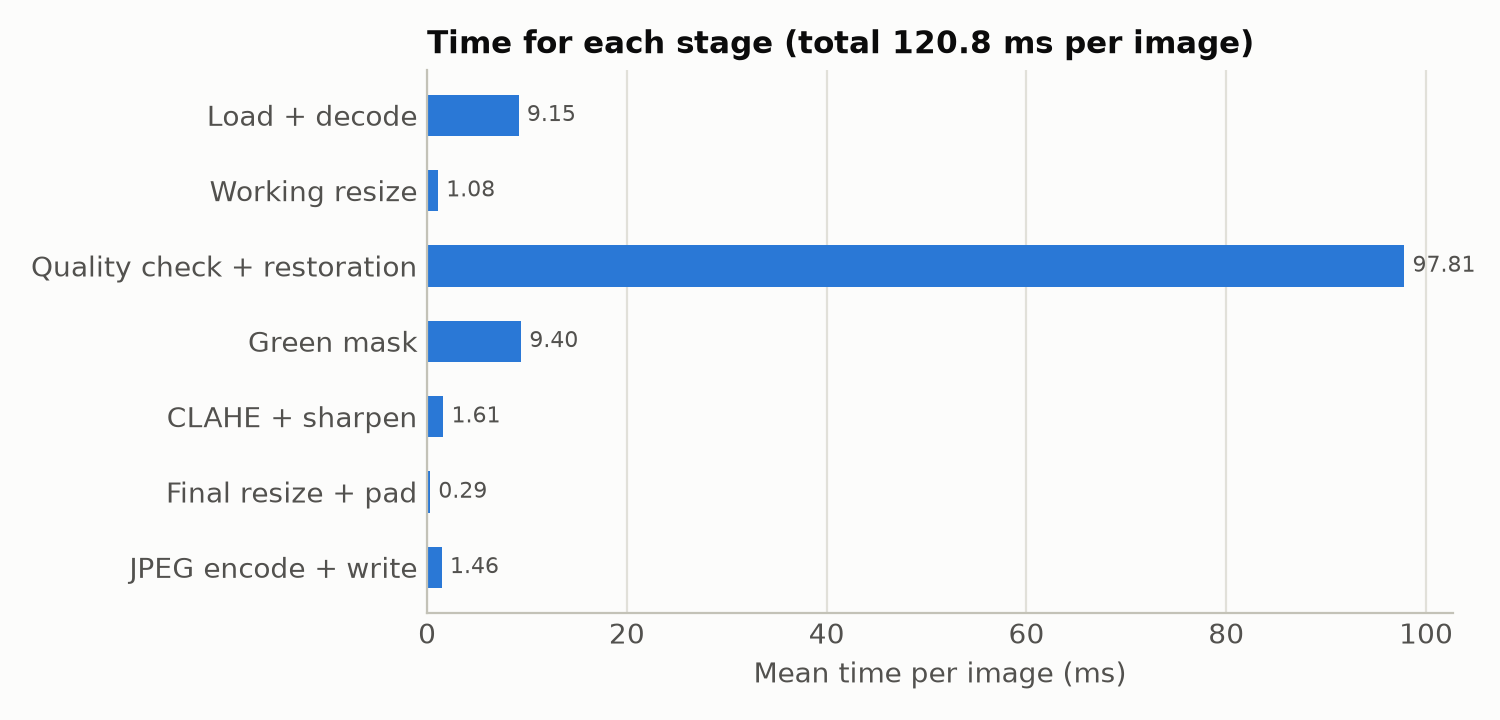
\includegraphics[width=0.66\textwidth]{time_per_stage.png}
\caption{Mean time for each stage.}
\label{fig:timing}
\end{figure}

\subsection{Quality assessment and restoration}
The quality check flagged 128 of the 590 images (21.7\%) with a BRISQUE score above 30. For these images the mean score fell from 39.11 to 15.88 after the selected filter (Table~\ref{tab:iqa}, Figure~\ref{fig:brisque}). The reference paper reports 40.75 to 16.17 for its hand-selected filters on 12 images, so the automatic selection reaches a comparable level on a set that is ten times larger. Over all 590 images the mean score fell from 19.51 to 14.47.

\begin{table}[H]
\centering
\caption{BRISQUE before and after the restoration stage (lower is better).}
\label{tab:iqa}
\small
\begin{tabular}{lrrrrrr}
\toprule
 & & & \multicolumn{2}{c}{All images} & \multicolumn{2}{c}{Flagged images} \\
\cmidrule(lr){4-5}\cmidrule(lr){6-7}
Class & Images & Flagged & Before & After & Before & After \\
\midrule
Black aphid  & 100 & 28 & 21.16 & 13.69 & 38.56 & 11.86 \\
Green aphid  &  90 & 14 & 18.84 & 13.76 & 45.24 & 12.59 \\
Mealybug     & 100 & 19 & 17.71 & 13.77 & 40.77 & 20.00 \\
Red mite     & 100 & 16 & 19.70 & 17.01 & 36.79 & 19.97 \\
Whitefly     & 100 & 20 & 18.89 & 16.20 & 37.83 & 24.41 \\
Yellow aphid & 100 & 31 & 20.69 & 12.32 & 37.86 & 10.86 \\
\midrule
Total        & 590 & 128 & 19.51 & 14.47 & 39.11 & 15.88 \\
\bottomrule
\end{tabular}
\end{table}

\begin{figure}[H]
\centering
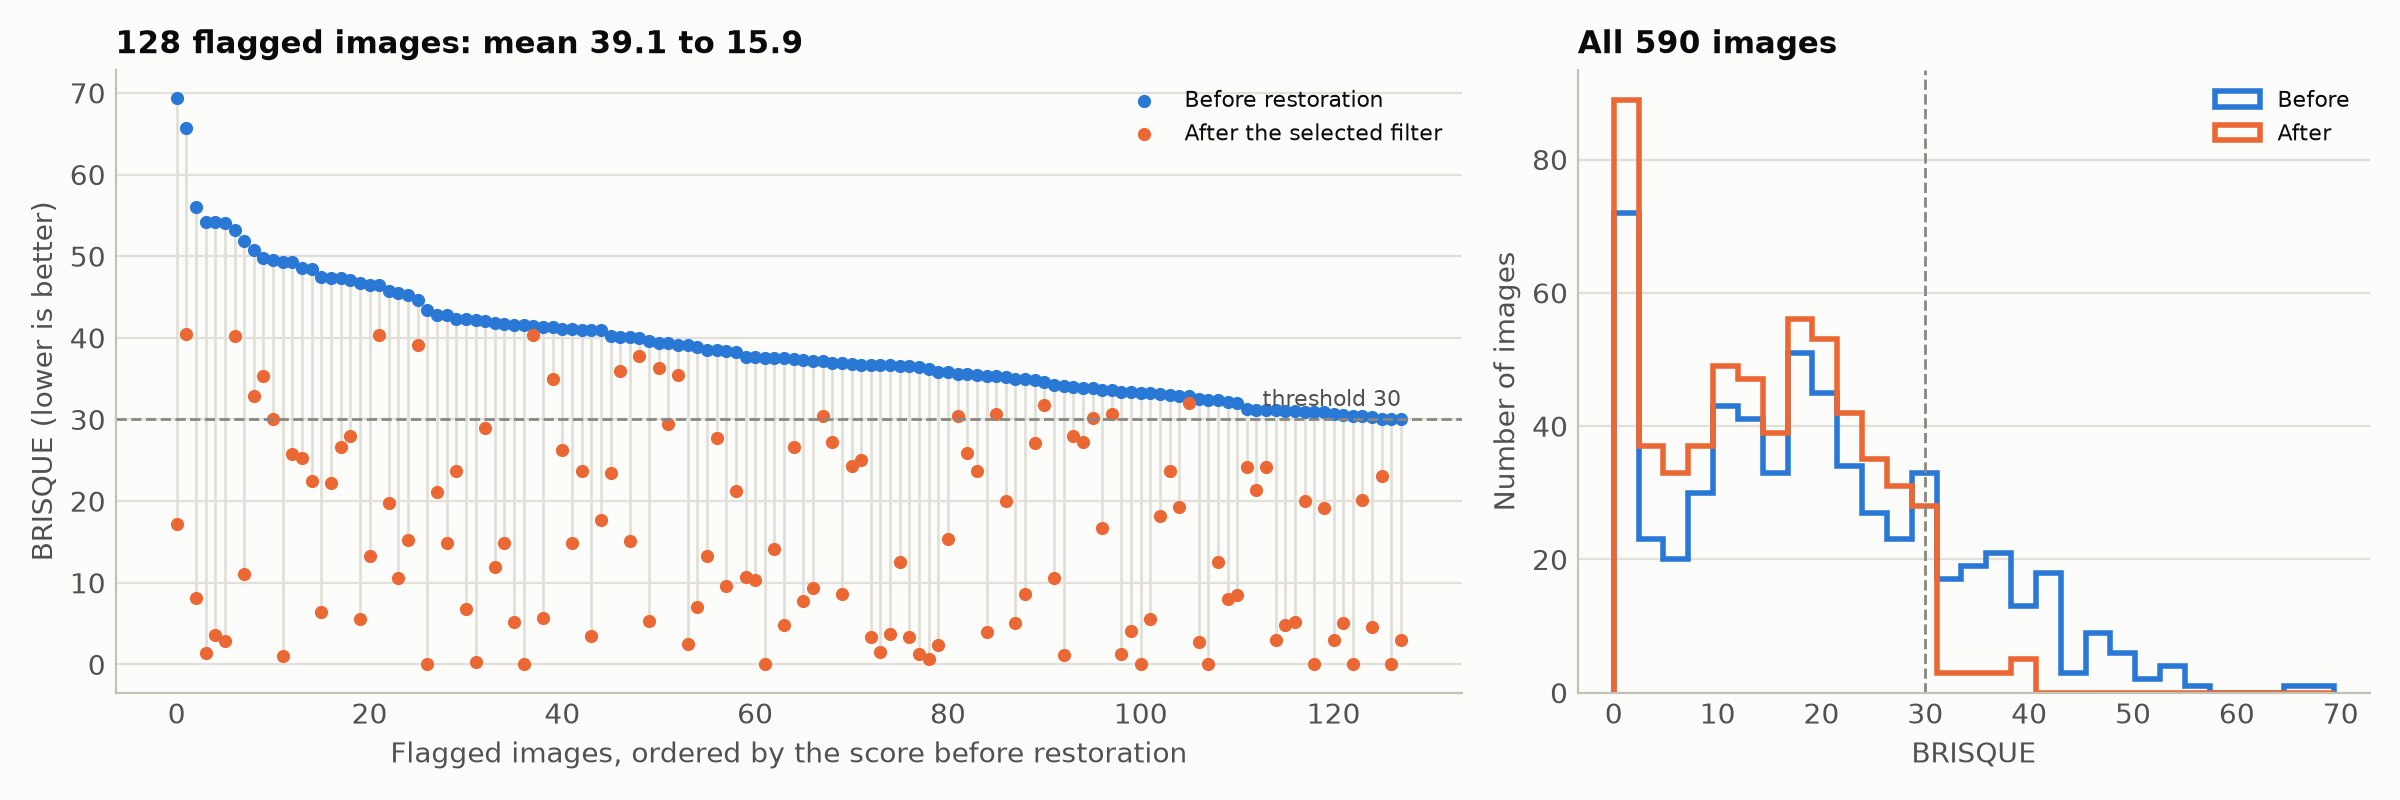
\includegraphics[width=\textwidth]{brisque_before_after.png}
\caption{Left: BRISQUE of each flagged image before and after the selected filter. Right: distribution over all images.}
\label{fig:brisque}
\end{figure}

Table~\ref{tab:filters} shows which filter was selected. No single filter is best for all images, which agrees with the paper. The Wiener filter was selected for 74 images and unsharp masking for 48. The smoothing filters (median, Gaussian, total variation) were almost never selected and gave worse mean scores than the unchanged image. The reason is the dataset: these photographs are limited by soft focus and not by noise, so smoothing removes detail that BRISQUE counts as quality. Figure~\ref{fig:restore} shows the candidates for four images.

\begin{table}[H]
\centering
\caption{Filter selection for the 128 flagged images.}
\label{tab:filters}
\small
\begin{tabular}{lrr}
\toprule
Filter & Times selected & Mean BRISQUE on all flagged images \\
\midrule
No change        &  0 & 39.11 \\
Median           &  2 & 51.28 \\
Gaussian         &  0 & 58.66 \\
Wiener           & 74 & 18.54 \\
Richardson--Lucy &  3 & 25.04 \\
Total variation  &  1 & 66.80 \\
Unsharp masking  & 48 & 20.77 \\
\bottomrule
\end{tabular}
\end{table}

\begin{figure}[H]
\centering
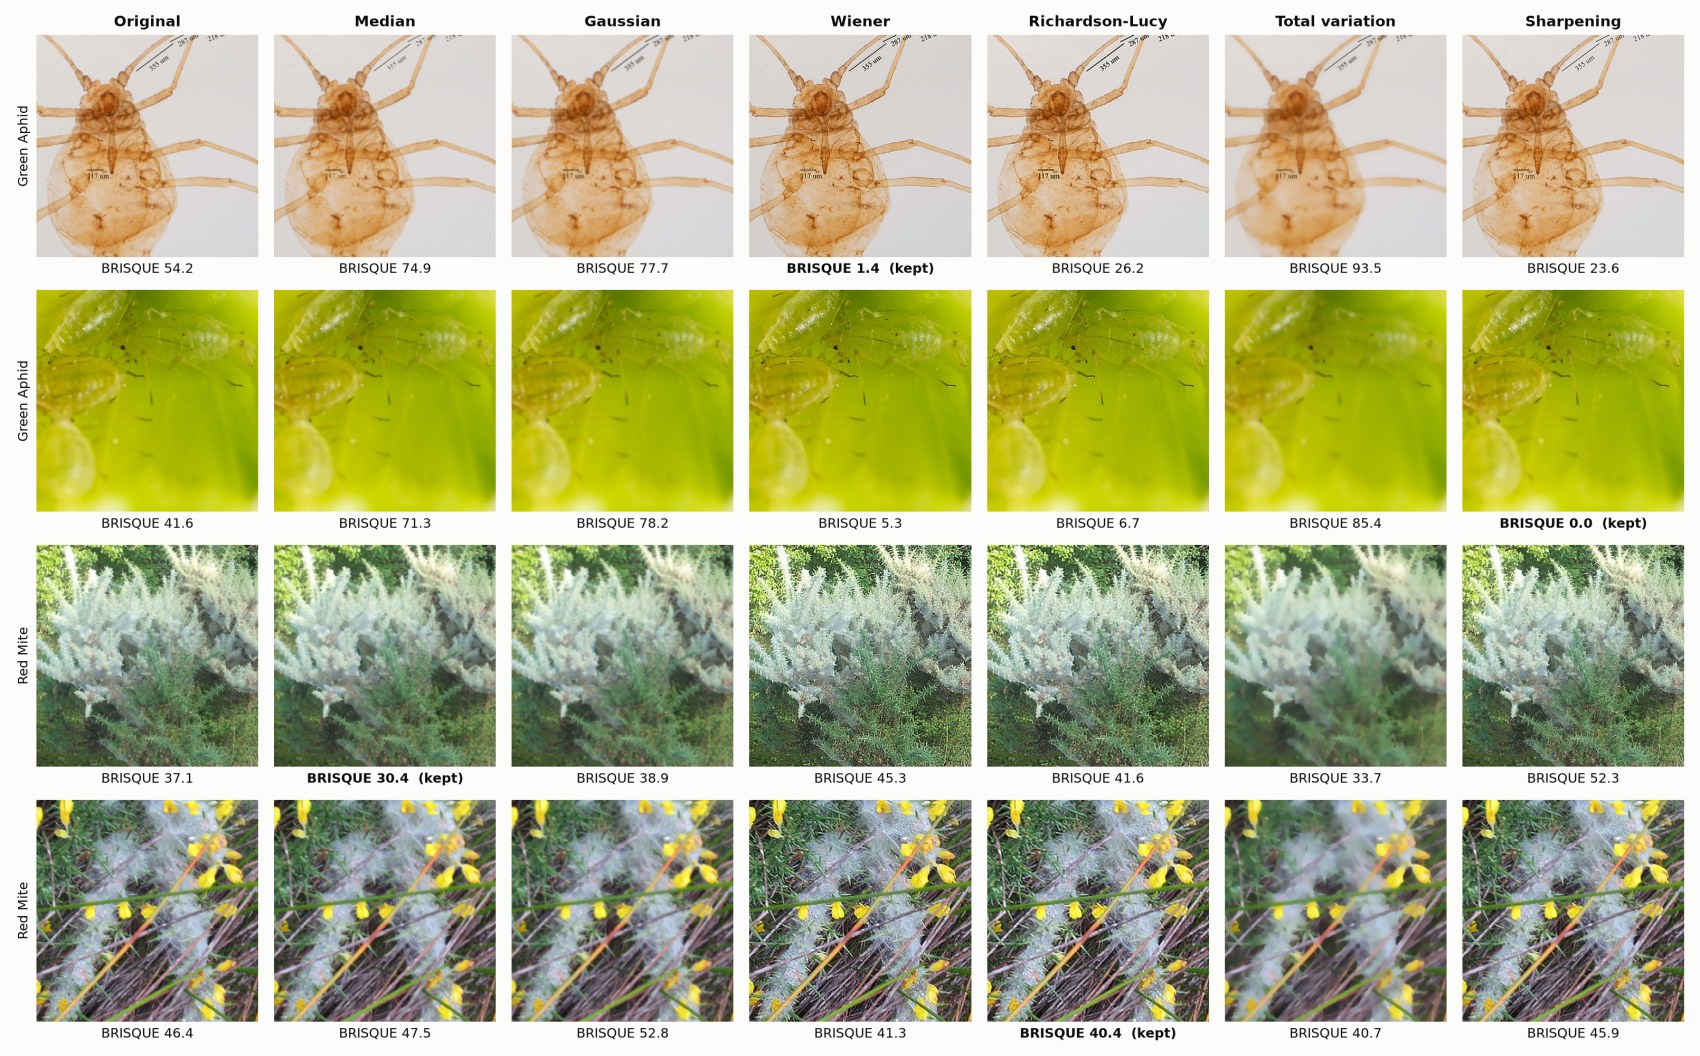
\includegraphics[width=\textwidth]{restoration_examples.jpg}
\caption{Candidate filters on four flagged images (centre crop). The kept result is marked.}
\label{fig:restore}
\end{figure}

\subsection{Controlled degradation test}
Table~\ref{tab:degradation} and Figure~\ref{fig:degpsnr} give the result of the test with known clean images. This test answers a question that BRISQUE cannot answer alone: is the selected filter closer to the true image?

\begin{table}[H]
\centering
\caption{Mean PSNR (dB) of each filter on 60 degraded images. In brackets: the number of images for which BRISQUE selected the filter / for which the filter had the best PSNR.}
\label{tab:degradation}
\footnotesize
\setlength{\tabcolsep}{4pt}
\begin{tabular}{lccc}
\toprule
Filter & Gaussian blur & Gaussian noise & Salt-and-pepper \\
\midrule
Degraded (no filter) & 31.00 (0 / 1)  & 24.82 (1 / 0)  & 18.95 (0 / 0) \\
Median               & 30.87 (0 / 4)  & 30.06 (58 / 0) & \textbf{35.03} (59 / 60) \\
Gaussian             & 30.37 (0 / 0)  & \textbf{31.43} (0 / 31) & 27.91 (0 / 0) \\
Wiener               & 31.01 (45 / 0) & 20.89 (0 / 0)  & 15.62 (0 / 0) \\
Richardson--Lucy     & \textbf{32.32} (12 / 55) & 22.46 (1 / 0) & 17.96 (1 / 0) \\
Total variation      & 28.72 (0 / 0)  & \textbf{31.43} (0 / 29) & 23.69 (0 / 0) \\
Unsharp masking      & 31.24 (3 / 0)  & 21.56 (0 / 0)  & 18.60 (0 / 0) \\
\midrule
PSNR, BRISQUE-selected & 31.46 & 29.93 & 34.89 \\
PSNR, best filter per image & 32.36 & 31.74 & 35.03 \\
SSIM, degraded to selected & 0.866 to 0.876 & 0.614 to 0.828 & 0.388 to 0.935 \\
\bottomrule
\end{tabular}
\end{table}

\begin{figure}[H]
\centering
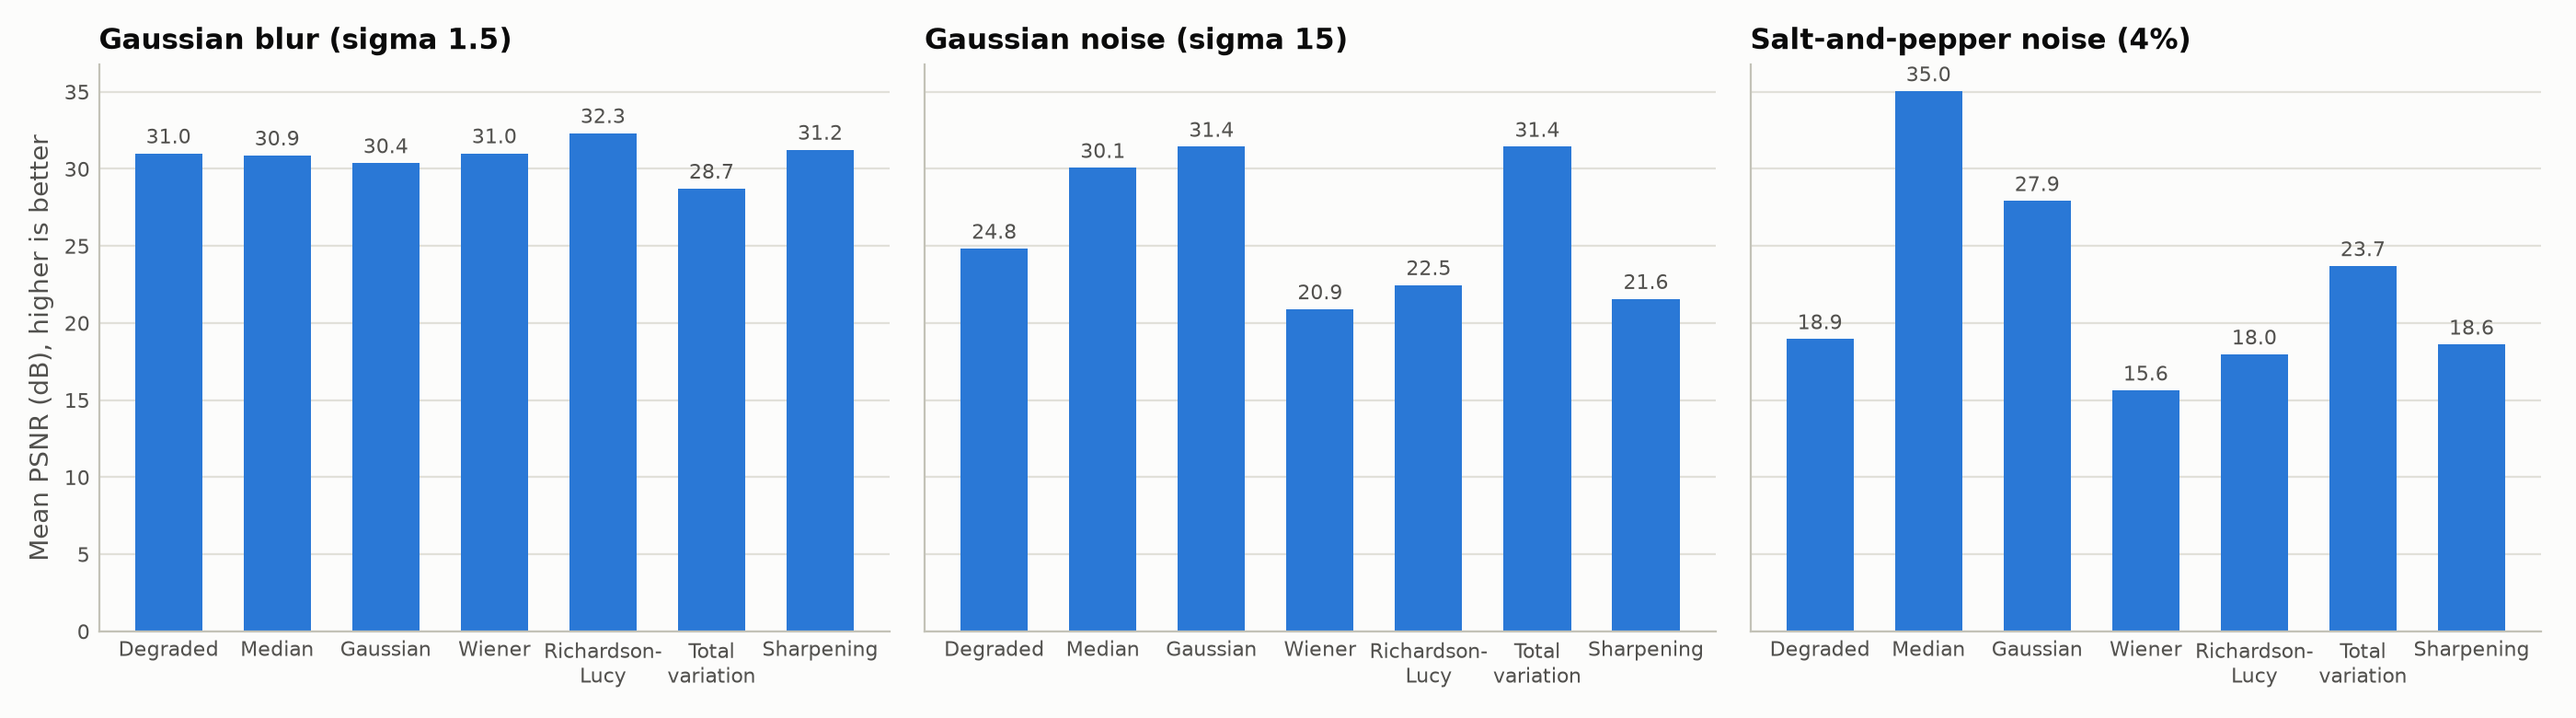
\includegraphics[width=\textwidth]{degradation_psnr.png}
\caption{Mean PSNR of each filter for each type of degradation.}
\label{fig:degpsnr}
\end{figure}

The selection always chose the correct family of filter: a deblurring filter for all 60 blurred images, and a smoothing filter for 58 of 60 noisy images and 59 of 60 impulse-noise images. It chose a deblurring filter for a noisy image in only 2 of 120 cases. The selected filter raised PSNR in all three cases: by 0.46~dB for blur, 5.11~dB for Gaussian noise and 15.94~dB for salt-and-pepper noise. Inside the correct family, the selected filter was not always the one with the best PSNR: BRISQUE preferred the Wiener filter where Richardson--Lucy was closer to the truth, and the median filter where the Gaussian filter was closer. The cost of this is 0.9~dB for blur and 1.8~dB for Gaussian noise. Figure~\ref{fig:degex} shows one example of each case.

\begin{figure}[H]
\centering
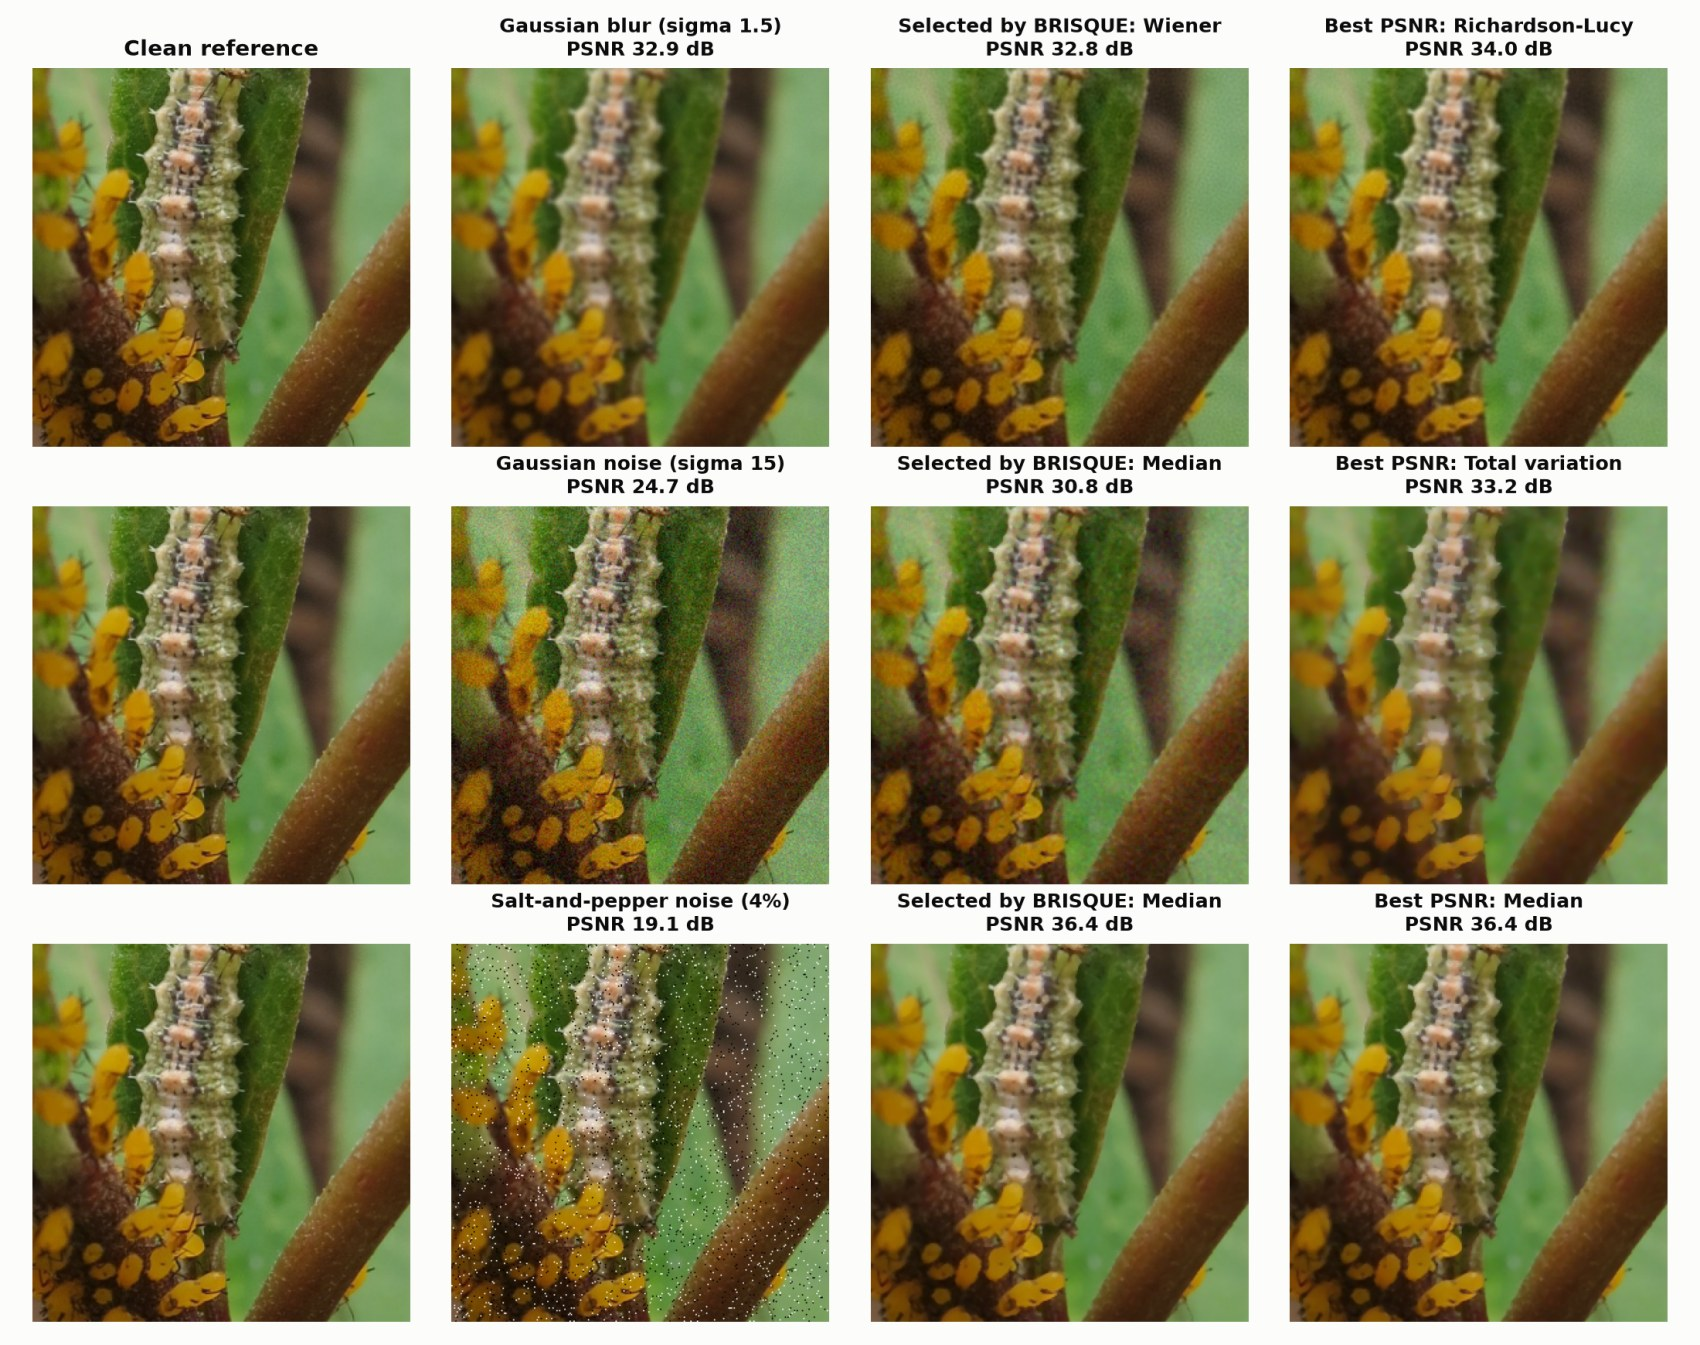
\includegraphics[width=0.86\textwidth]{degradation_examples.jpg}
\caption{One clean image with each degradation, the BRISQUE-selected result and the result with the best PSNR (centre crop).}
\label{fig:degex}
\end{figure}

\subsection{Enhancement and comparison with baseline methods}
Table~\ref{tab:baseline} compares the five versions. Figure~\ref{fig:clahe} shows why CLAHE was selected over global histogram equalisation, and Figure~\ref{fig:basevis} shows the versions side by side.

\begin{table}[H]
\centering
\caption{Baseline comparison, mean over 590 images at $512\times512$: RMS contrast, entropy in bits, sharpness as Laplacian variance, BRISQUE, and total compressed size. Version E is measured on foreground pixels only.}
\label{tab:baseline}
\small
\begin{tabular}{lrrrrr}
\toprule
Version & Contrast & Entropy & Sharpness & BRISQUE & Size (MB) \\
\midrule
A: resize only                      & 43.12 & 7.041 &  4832 & 18.74 & 23.50 \\
B: global histogram equalisation    & 70.70 & 7.868 & 15326 & 15.13 & 32.31 \\
C: CLAHE only                       & 51.46 & 7.460 & 12862 & 13.69 & 31.54 \\
D: restoration + CLAHE + sharpening & 52.58 & 7.496 & 23535 & 12.14 & 35.47 \\
E: full pipeline (with mask)        & 55.66 & 7.522 & 23421 & --    & 30.73 \\
\bottomrule
\end{tabular}
\end{table}

\begin{figure}[H]
\centering
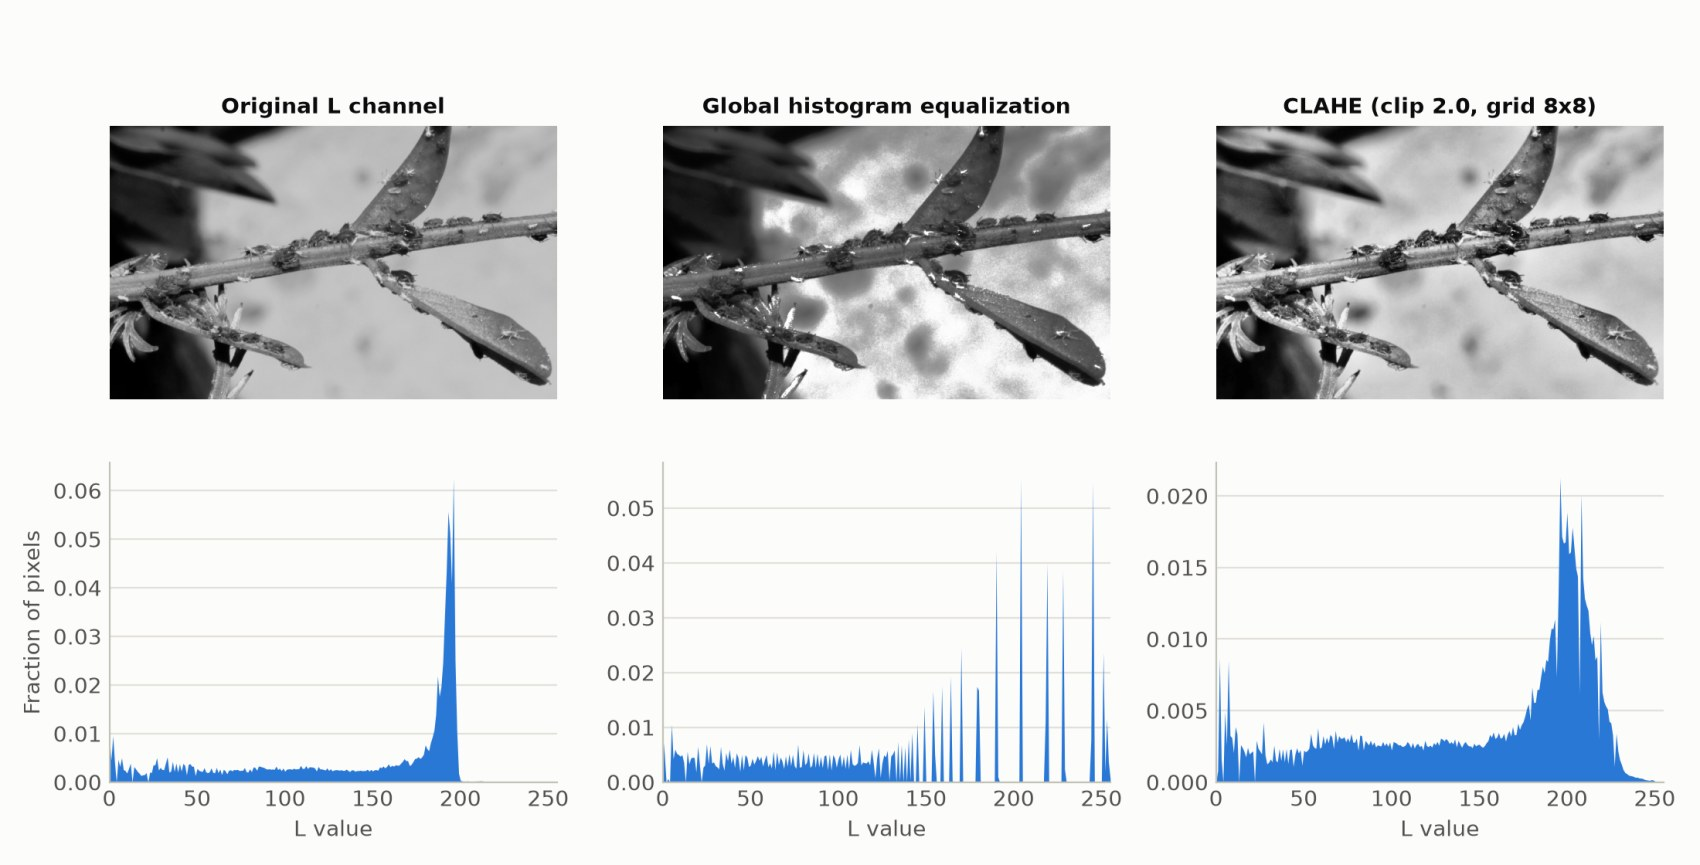
\includegraphics[width=0.92\textwidth]{clahe_histogram.jpg}
\caption{Lightness channel and its histogram: original, global histogram equalisation, and CLAHE.}
\label{fig:clahe}
\end{figure}

Global equalisation gives the highest contrast and entropy numbers, but Figure~\ref{fig:clahe} shows what those numbers hide: the smooth background becomes blotchy, and the histogram has gaps because grey levels were merged. CLAHE raises contrast by 19\% over the raw image and keeps a continuous histogram. Version D has the best BRISQUE score (12.14 against 18.74 for the raw image) and the highest sharpness. Against the raw image, the full pipeline raises RMS contrast by 29\% and entropy by 0.48~bits (Figure~\ref{fig:quality}).

\begin{figure}[H]
\centering
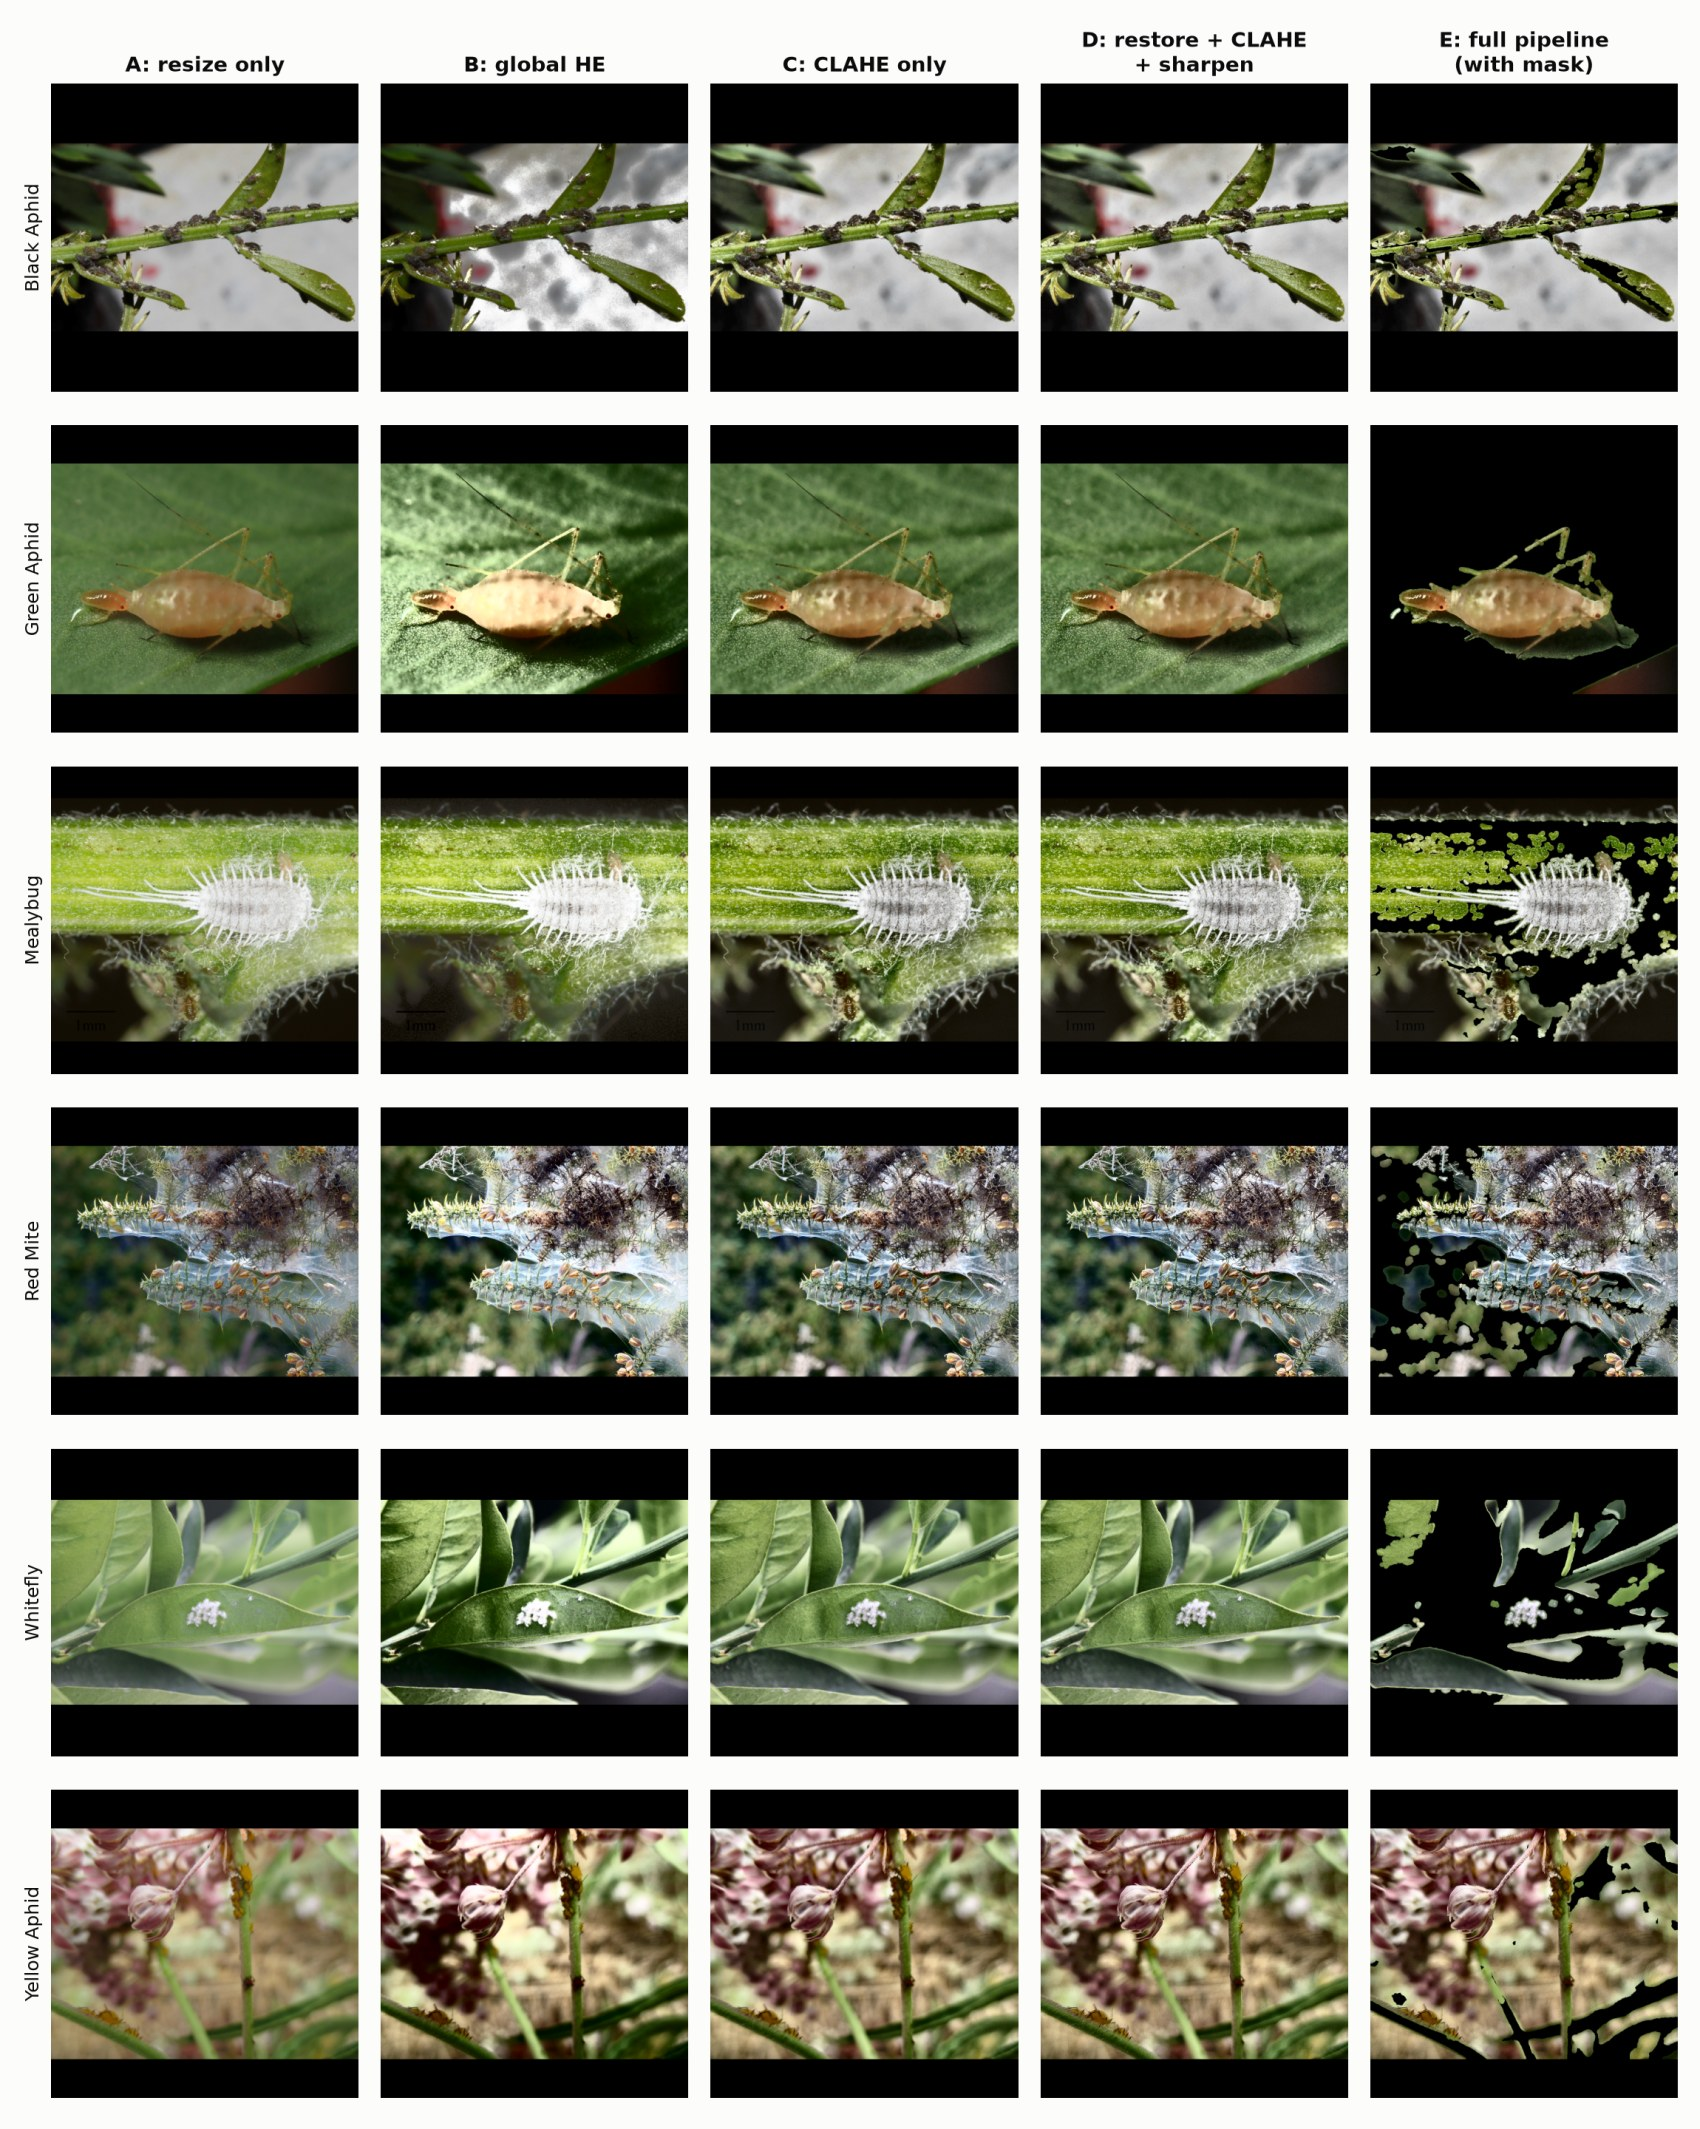
\includegraphics[width=\textwidth]{baseline_visual.jpg}
\caption{The five versions for one image of each class.}
\label{fig:basevis}
\end{figure}

\begin{figure}[H]
\centering
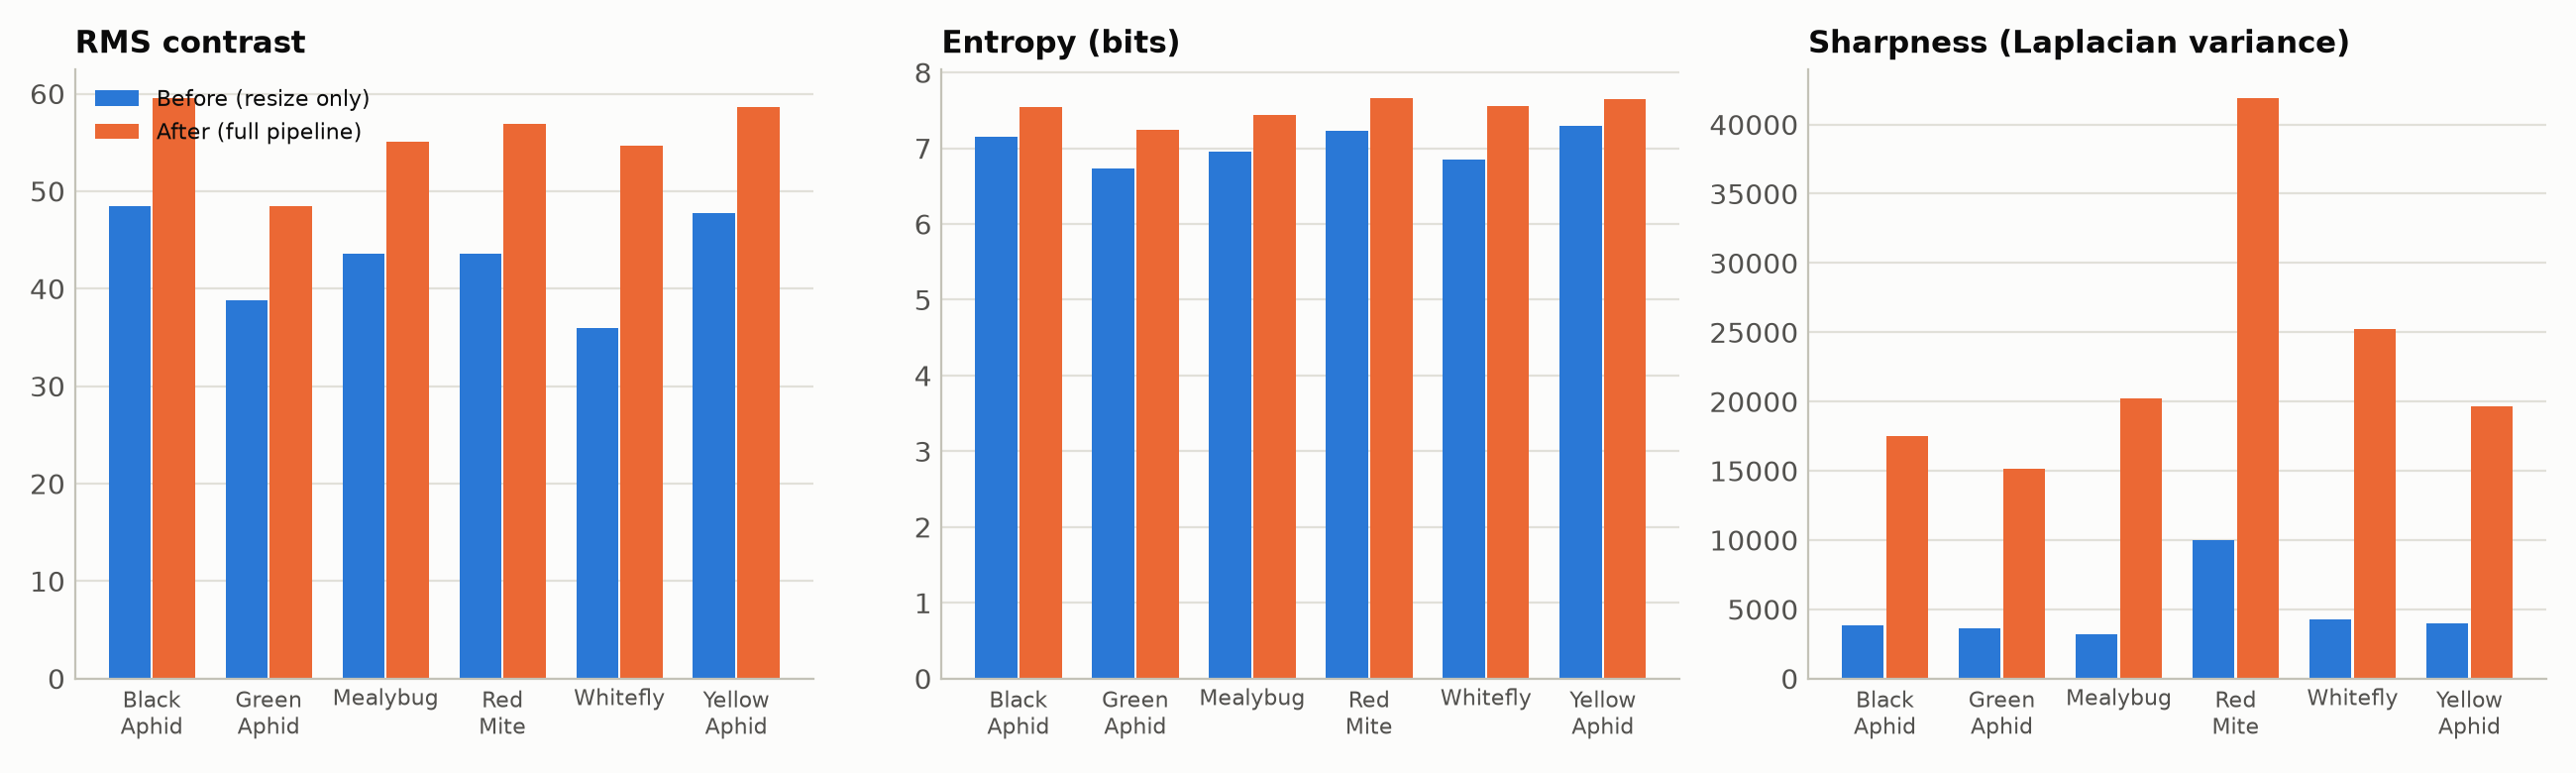
\includegraphics[width=\textwidth]{quality_before_after.png}
\caption{Quality metrics for each class before (resize only) and after (full pipeline).}
\label{fig:quality}
\end{figure}

\subsection{Background mask}
The mask was applied to 482 of 590 images (81.7\%). Of the others, 84 had no green background (less than 2\% green pixels) and 24 had almost no pixels near a dominant leaf colour. Where the mask was applied, it kept 63.7\% of the pixels on average (Figure~\ref{fig:fg}). The Otsu threshold on the chroma distance had a median of 9; the lower limit of 8 was used for 177 of 506 images and the upper limit of 25 for 6.

\begin{figure}[H]
\centering
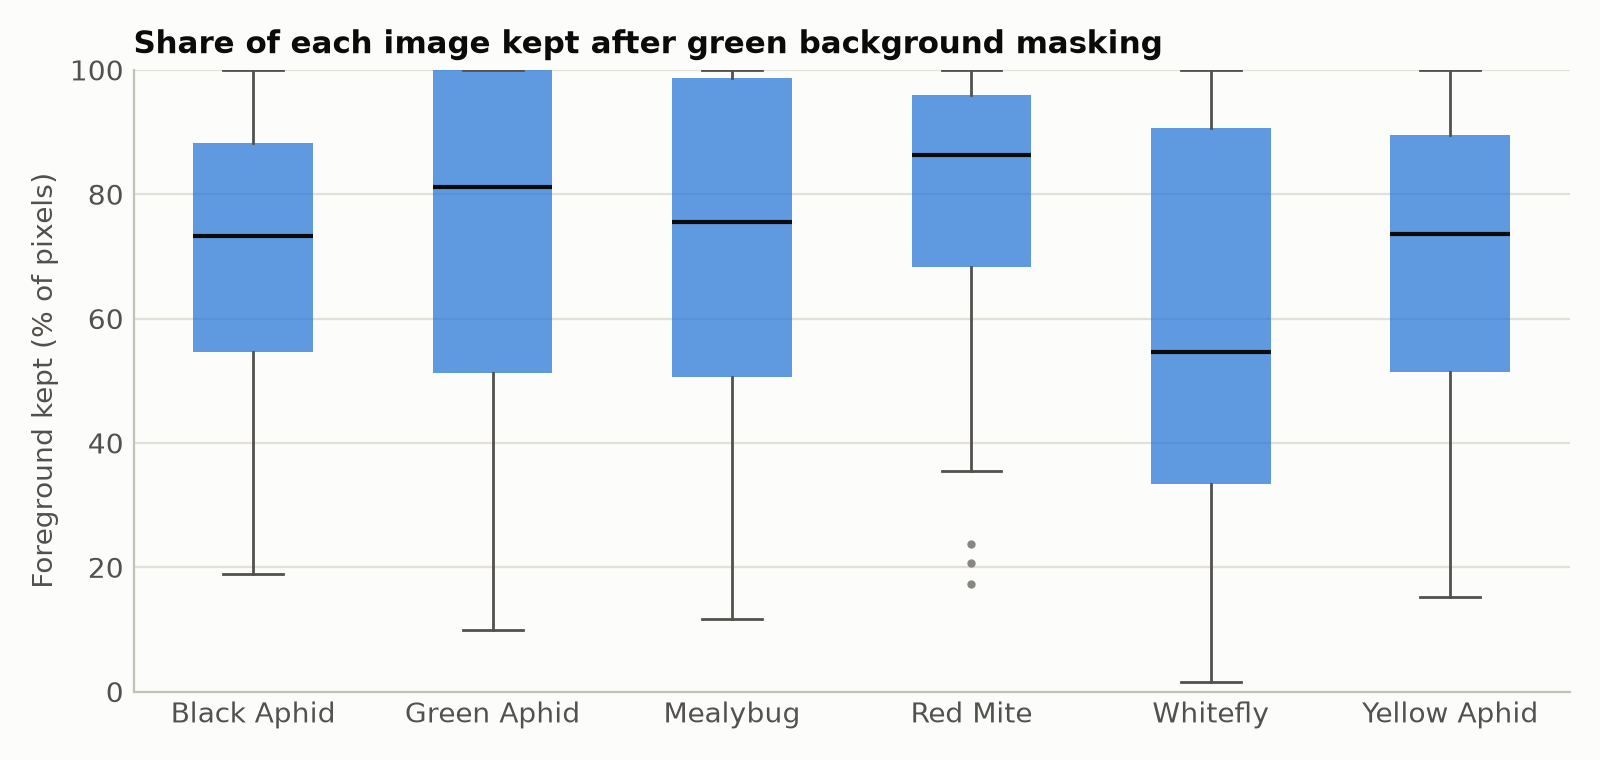
\includegraphics[width=0.66\textwidth]{foreground_fraction.png}
\caption{Share of each image that the mask kept, for each class.}
\label{fig:fg}
\end{figure}

\subsection{Classifier}
Table~\ref{tab:svm} gives the SVM result. The chance level for six classes is 16.7\%.

\begin{table}[H]
\centering
\caption{SVM accuracy and macro F1 (mean $\pm$ standard deviation over three repeats of 5-fold cross-validation).}
\label{tab:svm}
\small
\begin{tabular}{lcc}
\toprule
Version & Accuracy (\%) & Macro F1 \\
\midrule
A: resize only                      & $45.03 \pm 0.68$ & $0.450 \pm 0.006$ \\
C: CLAHE only                       & $44.18 \pm 1.44$ & $0.443 \pm 0.014$ \\
D: restoration + CLAHE + sharpening & $47.06 \pm 1.60$ & $0.471 \pm 0.016$ \\
E: full pipeline (with mask)        & $46.44 \pm 0.50$ & $0.465 \pm 0.005$ \\
\bottomrule
\end{tabular}
\end{table}

\begin{figure}[H]
\centering
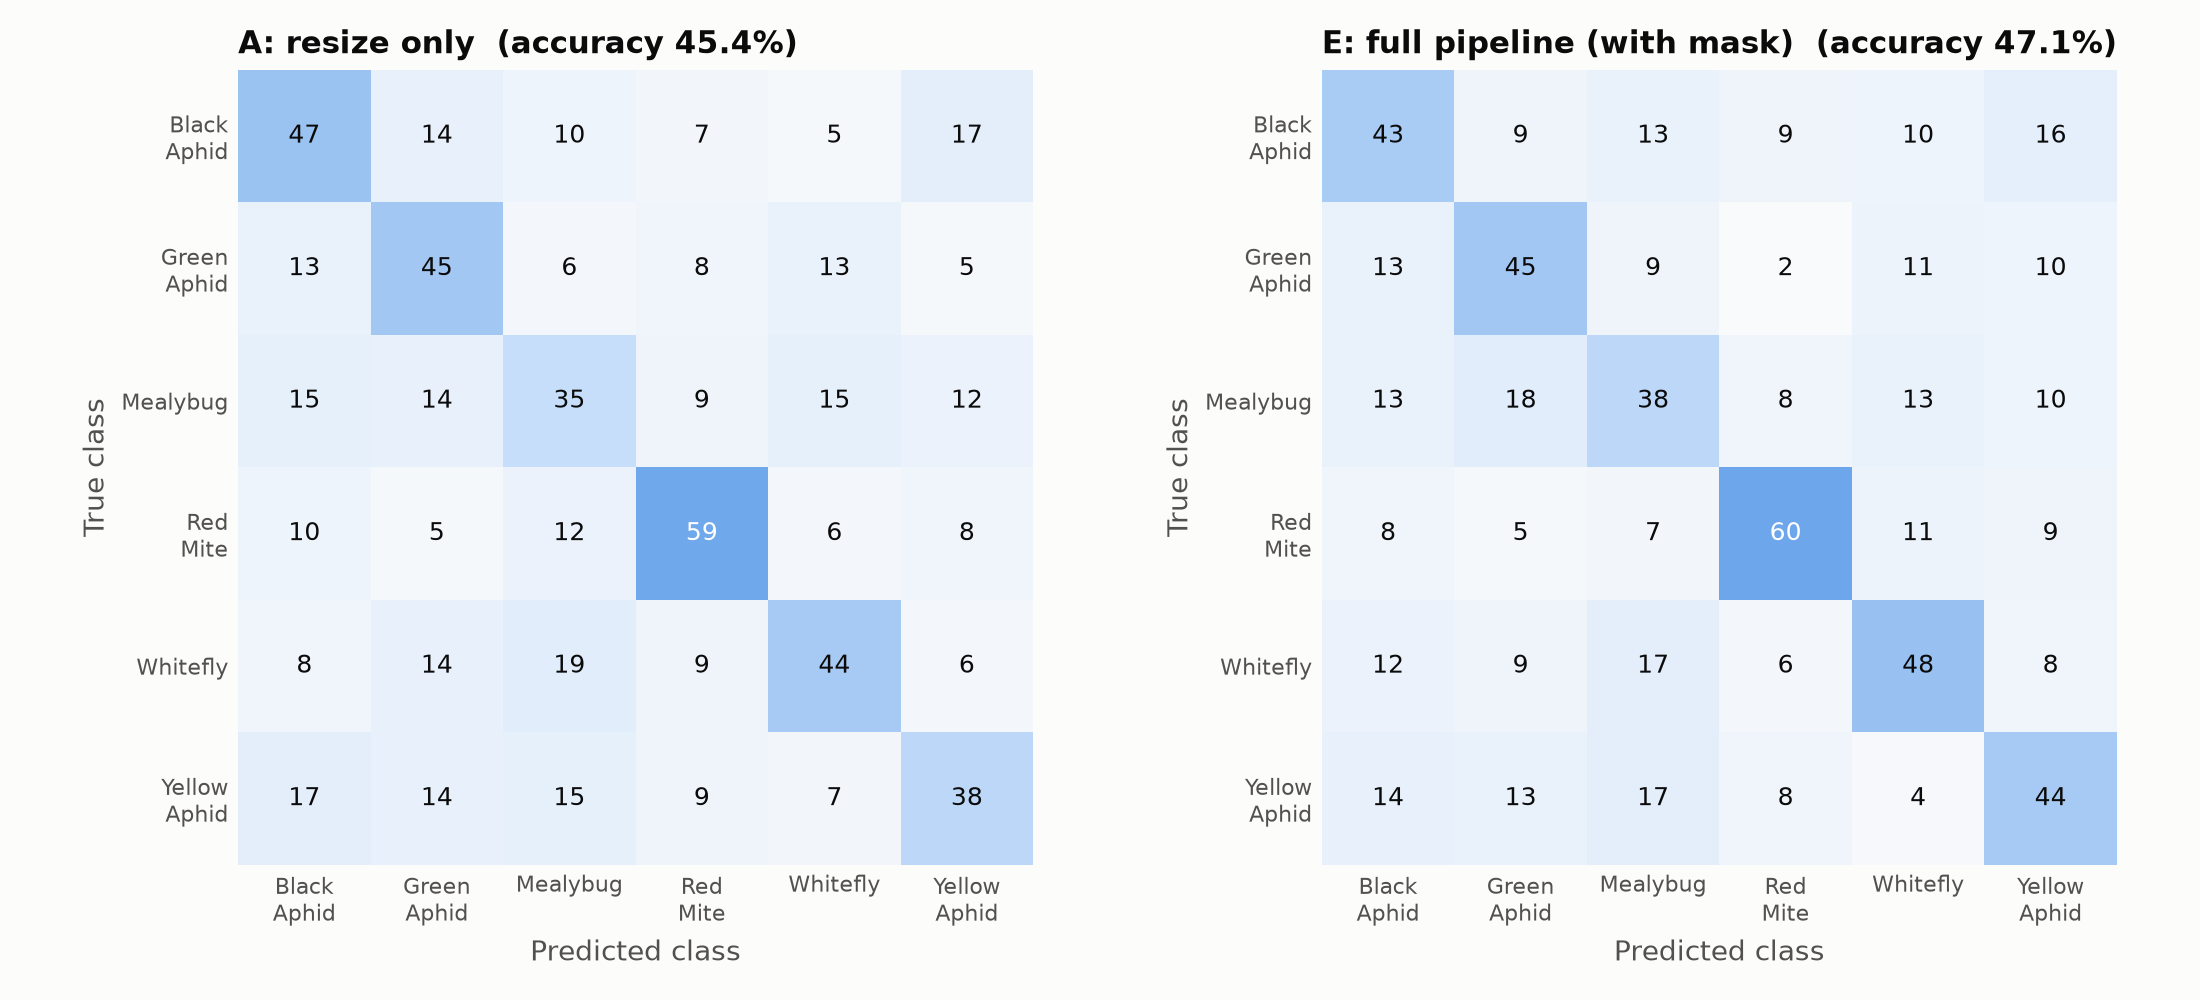
\includegraphics[width=0.95\textwidth]{confusion_matrices.png}
\caption{Confusion matrices for the raw images (A) and the full pipeline (E), first repeat.}
\label{fig:cm}
\end{figure}

The full pipeline is 1.4 percentage points above the raw images, and version D is 2.0 points above. The gain is about two standard deviations for E, so it is probably real, but it is small. In the per-class F1 scores of the first repeat, the pipeline improved five of the six classes (green aphid 0.459 to 0.476, mealybug 0.355 to 0.378, red mite 0.587 to 0.622, whitefly 0.463 to 0.487, yellow aphid 0.409 to 0.447) and made black aphid worse (0.448 to 0.424).

% ==============================================================================
\section{Discussion}

\subsection{Interpretation}
\paragraph{Where the storage reduction comes from.} Resizing and JPEG compression alone give 23.5~MB (version A), which is a 95.8\% reduction. The full pipeline gives 30.7~MB. Enhancement adds high-frequency detail that JPEG cannot remove, so versions C and D are larger (31.5 and 35.5~MB). The mask recovers part of that cost: it reduces the size by 13\% (35.5 to 30.7~MB), because a constant black region costs almost no bits. The storage objective is therefore met by normalisation; enhancement and masking are for the classifier, not for storage.

\paragraph{Quality-guided restoration works, with one reservation.} The stage reproduces the result of the reference paper on the BRISQUE score. The reservation is that a filter selected for the lowest BRISQUE must show a lower BRISQUE; the score is not independent evidence. The paper has the same construction. The controlled degradation test is the independent evidence: the selection found the correct type of filter in 177 of 180 cases and raised PSNR and SSIM in all three degradations. It also showed a weakness of BRISQUE as a selector: it rewards a sharp-looking result, so it prefers the Wiener filter to Richardson--Lucy and the median filter to the Gaussian filter, even where the other filter is closer to the true image.

\paragraph{The dataset decides which filter is useful.} On the real images, the median and Gaussian filters were selected twice in 128 cases and made the mean score worse. On the degraded images, they were the correct choice for every noisy image. A fixed denoising step, applied to all images, would have damaged this dataset: an early version of the pipeline did this and the mean BRISQUE rose from 19.5 to 35.8. This is direct support for the claim of the paper that preprocessing must follow a diagnosis of each image.

\paragraph{Enhancement and the classifier.} Contrast, entropy and sharpness all rose, and the classifier gained 1.4 to 2.0 points. The effect on the classifier is much smaller than the effect on the image metrics. Two reasons are likely. The features are global histograms of colour and texture, which do not use the location or shape of the pest. In addition, each species in this dataset lives on typical host plants, so the background carries class information; masking removes that shortcut, which is correct for a model that must work on other crops, but it does not raise accuracy inside this dataset.

\subsection{Comparison with the reference paper}
\begin{table}[H]
\centering
\caption{Reference paper and this work.}
\small
\begin{tabular}{p{3.3cm}p{5.6cm}p{5.6cm}}
\toprule
 & Jia et al.\ \cite{jia2025} & This work \\
\midrule
Dataset & 4 pest classes from IP102 \cite{wu2019} & 6 pest classes, 590 images \\
Quality metric & BRISQUE, PIQE, NIQE (MATLAB) & BRISQUE (OpenCV) \\
Images restored & 12 with BRISQUE $> 30$ & 128 with BRISQUE $> 30$ \\
Filters & Wiener, Lucy--Richardson, sharpening, damped least squares, Tikhonov, total variation & Wiener, Richardson--Lucy, sharpening, total variation, median, Gaussian \\
Filter selection & By hand for each image & Automatic, lowest BRISQUE \\
Mean BRISQUE & 40.75 $\rightarrow$ 16.17 & 39.11 $\rightarrow$ 15.88 \\
Validation with a reference & None & PSNR and SSIM on controlled degradations \\
Later stages & Clustering segmentation, edge detection, YOLOv5 detector & Colour mask, CLAHE, resize, JPEG, SVM classifier \\
\bottomrule
\end{tabular}
\end{table}

The damped least squares and Tikhonov filters of the paper were not implemented; both are regularised inverse filters of the same family as the Wiener filter. PIQE and NIQE are not in OpenCV and were not implemented. The paper does not give its filter parameters, so the parameters here are our own.

\subsection{Failure cases and limitations}
Figure~\ref{fig:fail} shows the extreme cases of the mask.

\begin{figure}[H]
\centering
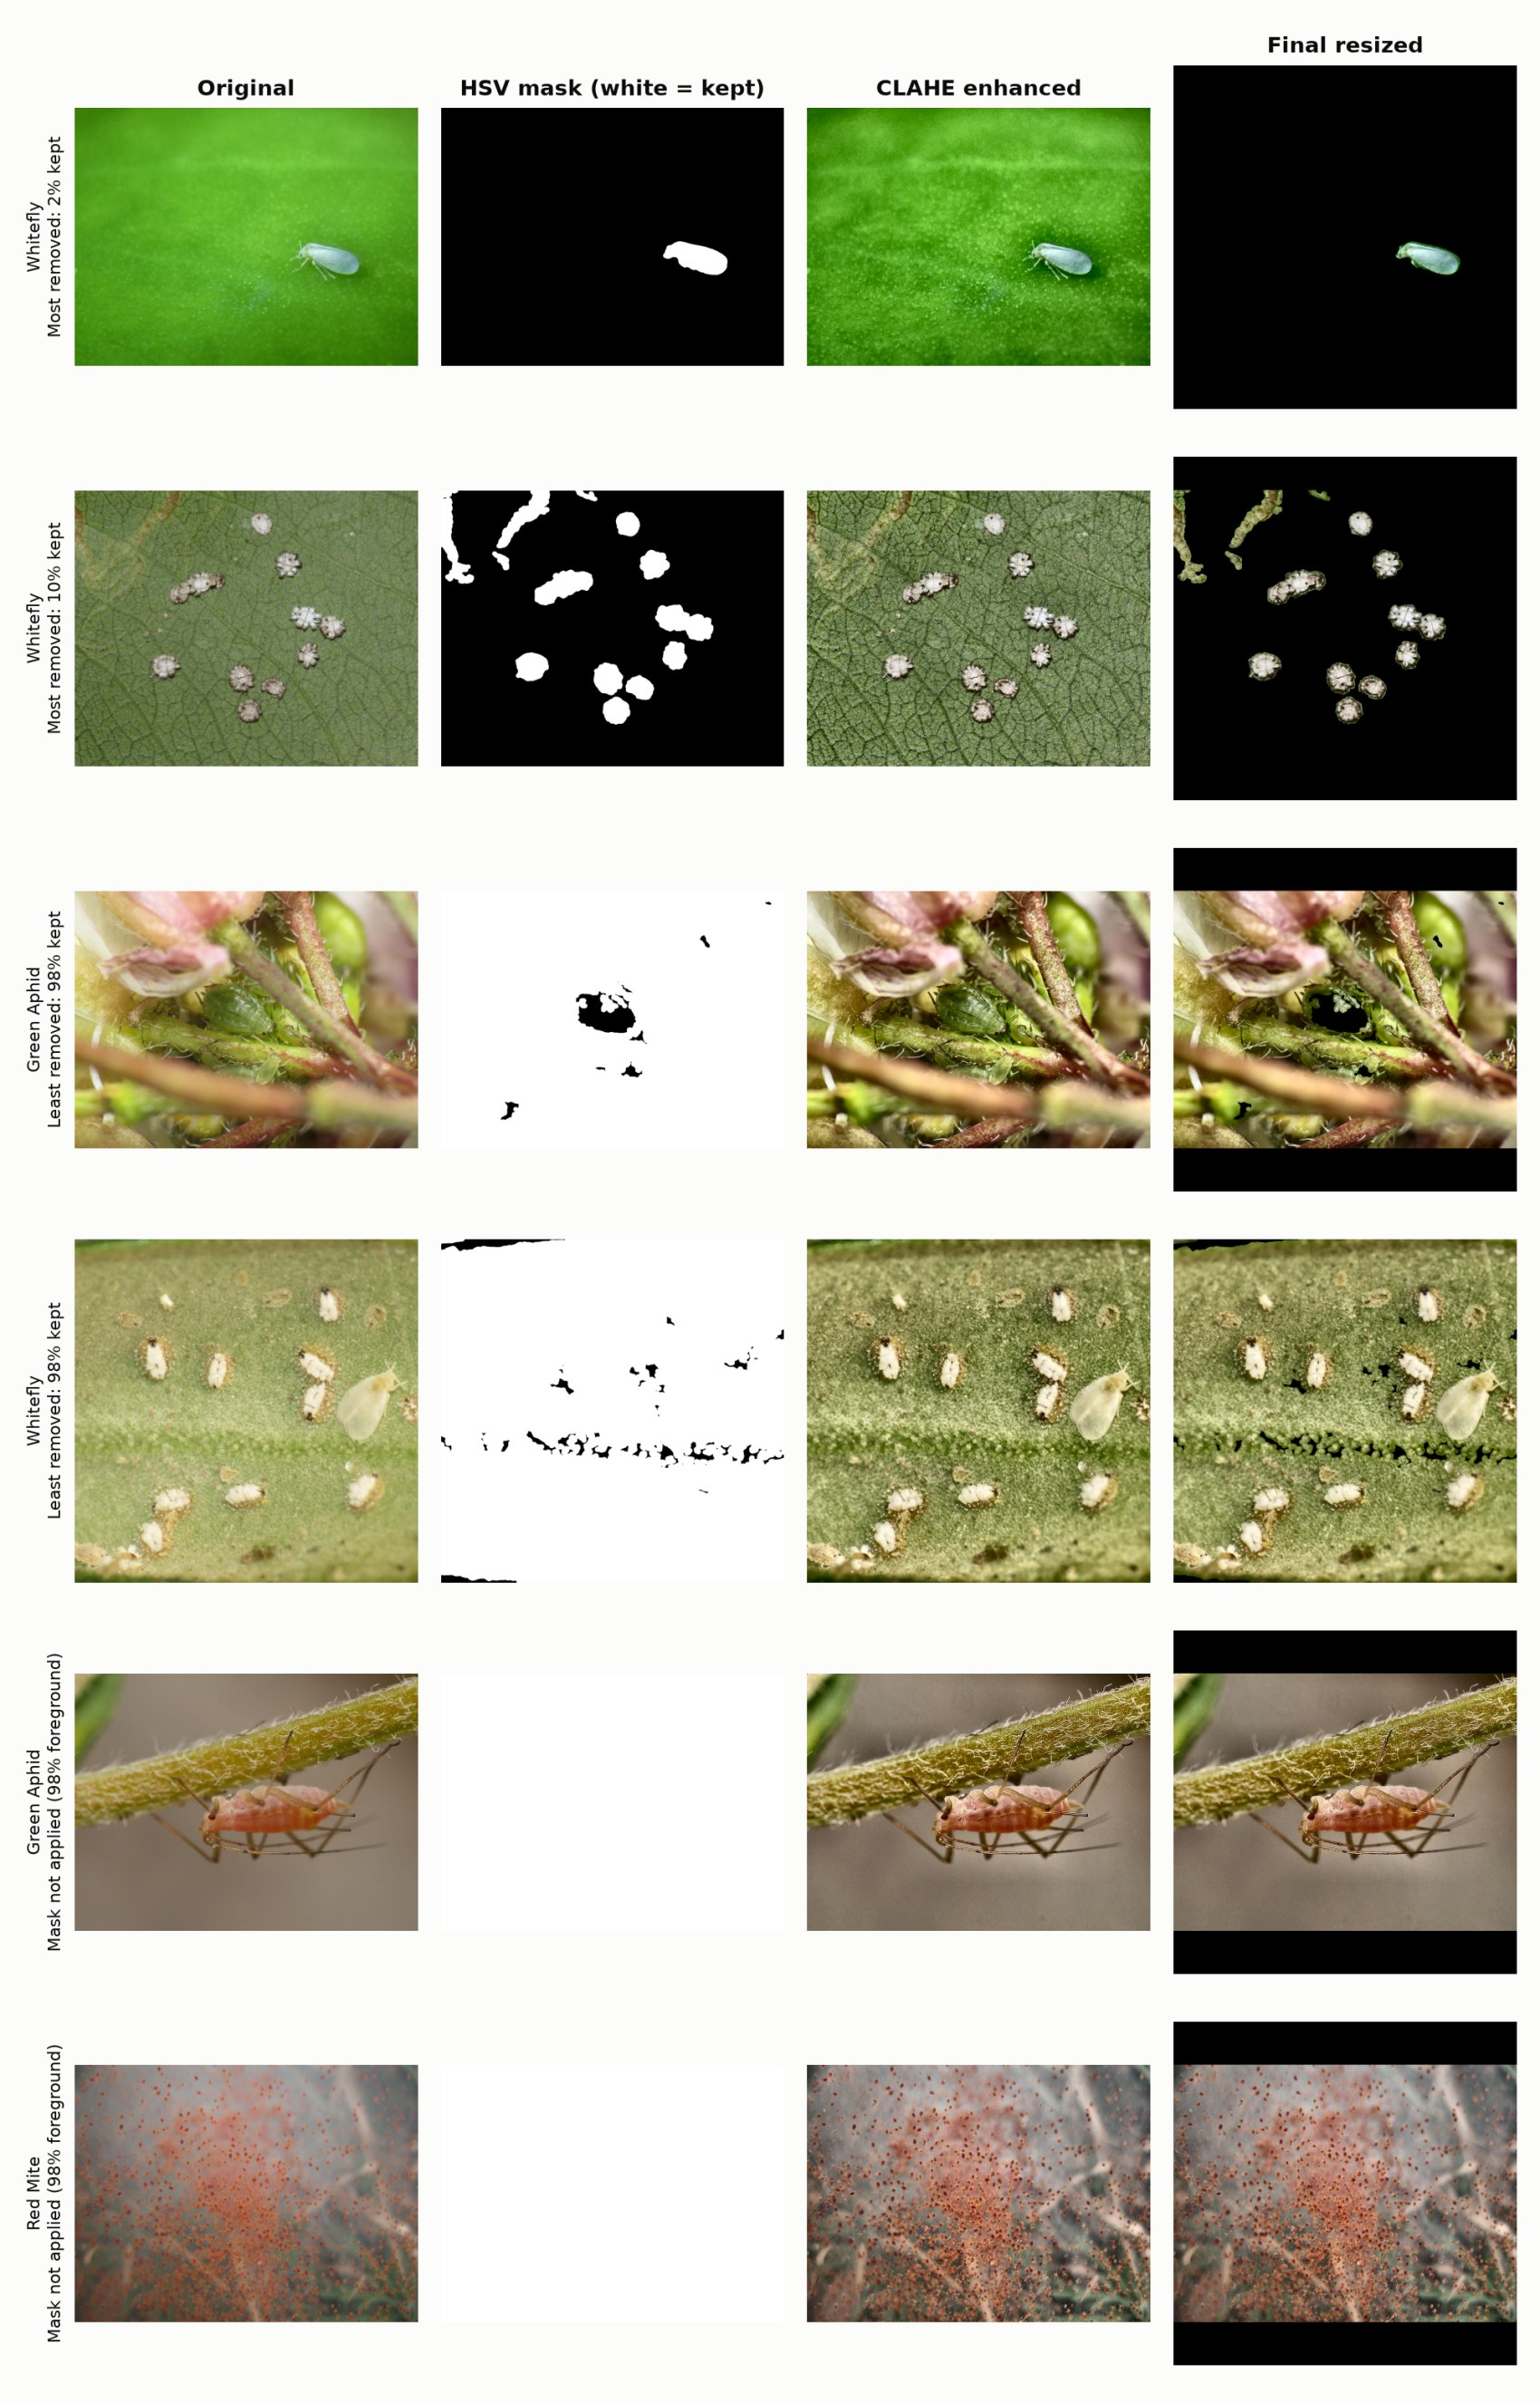
\includegraphics[width=0.74\textwidth]{mask_extreme_cases.jpg}
\caption{Extreme cases of the mask: the images with the most and the least background removed, and images where the mask was not applied.}
\label{fig:fail}
\end{figure}

\begin{itemize}[nosep]
\item \textbf{Green pest on a green plant.} A colour mask cannot separate a green aphid from the stem or leaf under it. In the third row of Figure~\ref{fig:fail} the aphid has the dominant green colour, so the mask removes the aphid and keeps the surroundings. Green aphid is also the class with the lowest share of masked images (64\%). Shape or texture information is necessary for this class.
\item \textbf{Background that is not green.} Soil, bark, sky, fingers and dry leaves are not removed, because the mask only models green.
\item \textbf{Assumed PSF.} The deblurring filters assume a Gaussian PSF with a fixed width. Motion blur or a different amount of defocus is not modelled, which limits the gain for blur (0.46~dB).
\item \textbf{Fixed threshold.} The BRISQUE threshold of 30 is taken from the paper and was not tuned. The BRISQUE model was trained on general photographs, not on macro images of insects.
\item \textbf{Time.} A flagged image takes about nine times longer than a good image. The paper names this cost as a limitation, and automatic selection does not remove it.
\item \textbf{Stand-in dataset.} The photographs are mostly of good quality and are taken by people who wanted a clear image of the insect. A dataset from a fixed field camera will have more noise and blur, more flagged images and a longer mean time.
\item \textbf{Classifier.} An SVM on global histograms is a weak model. The result shows the direction of the effect, not the accuracy that a convolutional network can reach.
\end{itemize}

% ==============================================================================
\section{Conclusion}

\subsection{Findings}
\begin{itemize}[nosep]
\item The pipeline reduced 590 images from 566.2~MB to 30.7~MB (94.6\%) at a mean of 121~ms for each image, and wrote $512\times512$ images sorted into six class folders.
\item Automatic, BRISQUE-guided filter selection reduced the mean score of the low-quality images from 39.1 to 15.9, comparable to the hand-tuned result of the reference paper (40.75 to 16.17).
\item With a known clean image, the selected filter raised PSNR by 0.5 to 15.9~dB and was of the correct type in 98\% of cases.
\item CLAHE and sharpening raised RMS contrast by 29\% and entropy by 0.48~bits, without the artefacts of global equalisation.
\item The mask based on the dominant leaf colour isolated pale and small pests that a plain green threshold removes.
\item The classifier gained 1.4 percentage points, a small effect.
\end{itemize}

\subsection{Objective achievement}
Objectives 1 to 5 were achieved. Objective 6 was achieved in the sense that the test was done; its answer is that the benefit to this simple classifier is small. The storage objective is met by resizing and compression, and the enhancement stages add size.

\subsection{Future improvements}
\begin{itemize}[nosep]
\item Estimate the blur width for each image, and add a motion-blur PSF, so that deconvolution matches the real degradation.
\item Replace the try-all-filters step with a direct mapping from BRISQUE features to a filter. This removes most of the time cost and is the direction that the paper proposes.
\item Add PIQE and NIQE and select with a combination of scores, to reduce the bias of BRISQUE towards sharp-looking results.
\item Add shape and texture cues, or GrabCut started from the colour mask, to keep green pests.
\item Crop to the bounding box of the foreground before the final resize, so that a small pest uses more of the $512\times512$ output.
\item Evaluate with a convolutional network and with the course dataset.
\end{itemize}

% ==============================================================================
\clearpage\renewcommand{\refname}{References}\addcontentsline{toc}{section}{References}
\makeatletter\renewcommand{\@biblabel}[1]{#1.}\makeatother
\begin{thebibliography}{99}
\small
\bibitem{jia2025} S. Jia, M. Horri Rezaei and B. Honarvar Shakibaei Asli, ``Enhancing pest detection in deep learning through a systematic image quality assessment and preprocessing framework,'' \textit{Journal of Experimental and Theoretical Analyses}, vol.~3, no.~4, art.~39, 2025. doi:10.3390/jeta3040039.
\bibitem{mittal2012} A. Mittal, A. K. Moorthy and A. C. Bovik, ``No-reference image quality assessment in the spatial domain,'' \textit{IEEE Transactions on Image Processing}, vol.~21, no.~12, pp.~4695--4708, 2012.
\bibitem{otsu1979} N. Otsu, ``A threshold selection method from gray-level histograms,'' \textit{IEEE Transactions on Systems, Man, and Cybernetics}, vol.~9, no.~1, pp.~62--66, 1979.
\bibitem{zuiderveld1994} K. Zuiderveld, ``Contrast limited adaptive histogram equalization,'' in \textit{Graphics Gems IV}, Academic Press, 1994, pp.~474--485.
\bibitem{richardson1972} W. H. Richardson, ``Bayesian-based iterative method of image restoration,'' \textit{Journal of the Optical Society of America}, vol.~62, no.~1, pp.~55--59, 1972.
\bibitem{lucy1974} L. B. Lucy, ``An iterative technique for the rectification of observed distributions,'' \textit{The Astronomical Journal}, vol.~79, pp.~745--754, 1974.
\bibitem{rudin1992} L. I. Rudin, S. Osher and E. Fatemi, ``Nonlinear total variation based noise removal algorithms,'' \textit{Physica D}, vol.~60, pp.~259--268, 1992.
\bibitem{chambolle2004} A. Chambolle, ``An algorithm for total variation minimization and applications,'' \textit{Journal of Mathematical Imaging and Vision}, vol.~20, pp.~89--97, 2004.
\bibitem{wang2004} Z. Wang, A. C. Bovik, H. R. Sheikh and E. P. Simoncelli, ``Image quality assessment: from error visibility to structural similarity,'' \textit{IEEE Transactions on Image Processing}, vol.~13, no.~4, pp.~600--612, 2004.
\bibitem{gonzalez2018} R. C. Gonzalez and R. E. Woods, \textit{Digital Image Processing}, 4th ed. Pearson, 2018.
\bibitem{ojala2002} T. Ojala, M. Pietik\"ainen and T. M\"aenp\"a\"a, ``Multiresolution gray-scale and rotation invariant texture classification with local binary patterns,'' \textit{IEEE Transactions on Pattern Analysis and Machine Intelligence}, vol.~24, no.~7, pp.~971--987, 2002.
\bibitem{cortes1995} C. Cortes and V. Vapnik, ``Support-vector networks,'' \textit{Machine Learning}, vol.~20, pp.~273--297, 1995.
\bibitem{wu2019} X. Wu, C. Zhan, Y.-K. Lai, M.-M. Cheng and J. Yang, ``IP102: a large-scale benchmark dataset for insect pest recognition,'' in \textit{Proc.\ IEEE/CVF Conference on Computer Vision and Pattern Recognition}, 2019, pp.~8787--8796.
\bibitem{inaturalist} iNaturalist, ``iNaturalist: research-grade observations.'' \url{https://www.inaturalist.org}.
\bibitem{opencv} G. Bradski, ``The OpenCV library,'' \textit{Dr.\ Dobb's Journal of Software Tools}, 2000.
\bibitem{scikit-image} S. van der Walt \textit{et al.}, ``scikit-image: image processing in Python,'' \textit{PeerJ}, vol.~2, e453, 2014.
\bibitem{scikit-learn} F. Pedregosa \textit{et al.}, ``Scikit-learn: machine learning in Python,'' \textit{Journal of Machine Learning Research}, vol.~12, pp.~2825--2830, 2011.
\end{thebibliography}

% ==============================================================================
\appendix
\renewcommand{\secword}{Appendix}
\addtocontents{toc}{\protect\renewcommand{\protect\cftsecpresnum}{Appendix }\protect\setlength{\protect\cftsecnumwidth}{6.4em}}
\section{Instructions for execution}

\subsection{Setup}
Python 3.11 or later is necessary.
\begin{lstlisting}[language=bash,numbers=none]
git clone https://github.com/shrayash25/dip-pest-preprocessing
cd dip-pest-preprocessing
python -m venv .venv
source .venv/bin/activate          # Windows: .venv\Scripts\activate
pip install -r requirements.txt
\end{lstlisting}

\subsection{Run}
\begin{lstlisting}[language=bash,numbers=none]
python run_all.py
\end{lstlisting}
This command needs no manual input. It does four steps:
\begin{enumerate}[nosep]
\item Downloads the dataset into \texttt{data/raw/<class>/} (skipped if the images are there). An internet connection is necessary for this step only.
\item Runs the pipeline. Processed images go to \texttt{data/processed/<class>/}; tables and figures go to \texttt{results/}.
\item Runs the controlled degradation test.
\item Runs the classifier comparison.
\end{enumerate}
A full run takes about four minutes after the download. To use a different dataset, put the images in \texttt{data/raw/<class name>/}, one folder for each class, before the command is run.

\subsection{Run on one folder of images}
\begin{lstlisting}[language=bash,numbers=none]
python run_all_once.py
\end{lstlisting}
This command runs all stages of the pipeline on each image in the folder \texttt{run-all-once} and writes the final images, one step plot for each image, \texttt{results.csv} and \texttt{summary.txt} to the folder \texttt{output} inside it. Class folders and the dataset download are not necessary.

\subsection{Inputs and dependencies}
\begin{itemize}[nosep]
\item \textbf{Images:} listed in \texttt{data/raw/ATTRIBUTION.csv} with the photographer, licence and source page of each image.
\item \textbf{BRISQUE model files:} \texttt{brisque\_model\_live.yml} and \texttt{brisque\_range\_live.yml} in the \texttt{models} folder, from the OpenCV contrib project.
\item \textbf{Libraries:} opencv-contrib-python-headless 5.1.0.95, numpy 2.5.5, matplotlib 3.11.2, scikit-image 0.26.0, scikit-learn 1.9.1.
\end{itemize}

\section{Complete scripts}
\begin{singlespace}
\subsection{run\_all.py}
\lstinputlisting{../run_all.py}
\subsection{pest\_pipeline.py}
\lstinputlisting{../pest_pipeline.py}
\subsection{degradation\_experiment.py}
\lstinputlisting{../degradation_experiment.py}
\subsection{classify\_eval.py}
\lstinputlisting{../classify_eval.py}
\subsection{figures.py}
\lstinputlisting{../figures.py}
\subsection{download\_dataset.py}
\lstinputlisting{../download_dataset.py}
\subsection{run\_all\_once.py}
\lstinputlisting{../run_all_once.py}
\end{singlespace}

\end{document}
